\documentclass[12pt,a4paper]{article}

\usepackage[kazakh,russian,english]{babel}
\usepackage{fontspec}
\setmainfont{Times New Roman}
\setsansfont{Arial}
\setmonofont{Courier New}

\addto\captionskazakh{%
  \renewcommand{\contentsname}{Мазмұны}%
  \renewcommand{\listfigurename}{Суреттер тізімі}%
  \renewcommand{\listtablename}{Кестелер тізімі}%
  \renewcommand{\figurename}{Сурет}%
  \renewcommand{\tablename}{Кесте}%
  \renewcommand{\refname}{Әдебиеттер тізімі}%
  \renewcommand{\abstractname}{Аннотация}%
  \renewcommand{\appendixname}{Қосымша}%
}

\usepackage{microtype}
\usepackage[a4paper,top=2.5cm,bottom=2.5cm,left=2.5cm,right=2.5cm,headheight=15pt]{geometry}
\usepackage{setspace}
\onehalfspacing

\usepackage{graphicx}
\graphicspath{{figures/}}
\usepackage{float}
\usepackage[section]{placeins}
\usepackage{booktabs}
\usepackage{multirow}
\usepackage{longtable}
\usepackage{caption}
\captionsetup{labelsep=period}

\usepackage{amsmath,amssymb}
\usepackage[colorlinks=true,linkcolor=black,citecolor=blue,urlcolor=blue]{hyperref}

\usepackage{fancyhdr}
\pagestyle{fancy}
\fancyhf{}
\fancyhead[R]{\thepage}
\renewcommand{\headrulewidth}{0pt}

\setcounter{tocdepth}{2}
\setcounter{secnumdepth}{2}

\begin{document}

\section*{Аннотация}
\addcontentsline{toc}{section}{Аннотация}

Бұл зерттеу Алматы қаласындағы PM2.5 және PM10 концентрацияларын машиналық оқыту әдістері арқылы болжауға арналған. 2024–2025 жылдар аралығындағы (қолда бар деректер) сағаттық деректер негізінде уақыттық қатарлар талданып, кешенді feature engineering жүргізілді. Деректерді алдын ала өңдеу кезеңінде жетіспейтін мәндер толықтырылды, аномалиялар анықталды және уақыт белгілері стандартталды. Болжау үшін Linear Regression, Ridge, Lasso, Random Forest және Gradient Boosting модельдері қолданылды. Модельдер уақыттық қатарларға арналған дұрыс кросс-валидация әдістемесімен (TimeSeriesSplit) бағаланды, деректердің ағып кетуін болдырмау қатаң сақталды. Gradient Boosting моделі PM2.5 және PM10 үшін ең жоғары дәлдікті көрсетті, naive persistence baseline-ден айтарлықтай жақсы нәтижелер берді. Feature importance талдауы лаг айнымалылары мен жылжымалы статистикалардың маңыздылығын растады. Нәтижелер Алматы қаласы үшін ауа сапасын болжау жүйелерін құруға, ерте ескерту механизмдерін әзірлеуге және қоғамдық денсаулық саясатын қолдауға қолданылуы мүмкін.

\textbf{Түйін сөздер:} ауа ластануы, PM2.5, PM10, машиналық оқыту, уақыттық қатар, Алматы, болжам, Gradient Boosting.

\vspace{1cm}

\selectlanguage{russian}
\section*{Аннотация}
\addcontentsline{toc}{section}{Аннотация (русский)}

Данное исследование посвящено прогнозированию концентраций PM2.5 и PM10 в городе Алматы с использованием методов машинного обучения. На основе почасовых данных за период 2024–2025 гг. (имеющиеся данные) проведен анализ временных рядов и комплексная инженерия признаков. На этапе предобработки данных были заполнены пропущенные значения, выявлены аномалии и стандартизированы временные метки. Для прогнозирования применялись модели Linear Regression, Ridge, Lasso, Random Forest и Gradient Boosting. Модели оценивались с использованием правильной кросс-валидации для временных рядов (TimeSeriesSplit), строго соблюдались принципы предотвращения утечки данных. Модель Gradient Boosting показала наивысшую точность для PM2.5 и PM10, значительно превосходя naive persistence baseline. Анализ важности признаков подтвердил значимость лаговых переменных и скользящих статистик. Результаты могут быть применены для построения систем прогнозирования качества воздуха, разработки механизмов раннего предупреждения и поддержки политики общественного здравоохранения для города Алматы.

\textbf{Ключевые слова:} загрязнение воздуха, PM2.5, PM10, машинное обучение, временные ряды, Алматы, прогнозирование, Gradient Boosting.

\selectlanguage{english}
\section*{Abstract}
\addcontentsline{toc}{section}{Abstract (English)}

This research focuses on forecasting PM2.5 and PM10 concentrations in Almaty city using machine learning methods. Based on hourly data for the period 2024–2025 (available data), time series analysis and comprehensive feature engineering were performed. During preprocessing, missing values were imputed, anomalies identified, and timestamps standardized. Linear Regression, Ridge, Lasso, Random Forest, and Gradient Boosting models were applied for forecasting. Models were evaluated using proper time series cross-validation (TimeSeriesSplit), with strict adherence to data leakage prevention principles. Gradient Boosting showed the highest accuracy for both PM2.5 and PM10, significantly outperforming the naive persistence baseline. Feature importance analysis confirmed the significance of lag variables and rolling statistics. Results can be applied to building air quality forecasting systems, developing early warning mechanisms, and supporting public health policy for Almaty city.

\textbf{Keywords:} air pollution, PM2.5, PM10, machine learning, time series, Almaty, forecasting, Gradient Boosting.

\selectlanguage{kazakh}

\newpage
\tableofcontents
\newpage
\listoffigures
\addcontentsline{toc}{section}{Суреттер тізімі}
\newpage
\listoftables
\addcontentsline{toc}{section}{Кестелер тізімі}
\newpage

\section{Кіріспе}

\subsection{Зерттеудің өзектілігі}

Ауа ластануы қазіргі заманғы қалалық ортаның ең маңызды экологиялық және әлеуметтік мәселелерінің бірі болып табылады. Дүниежүзілік денсаулық сақтау ұйымының (ДДҰ) деректері бойынша, әлемдегі қалалық халықтың үлкен бөлігі ауа сапасы нормативтік стандарттарға сәйкес келмейтін жағдайларда тұрады \cite{who2021}. Ауа ластануының қоғамдық денсаулыққа әсері – тыныс алу жолдарының аурулары, жүрек-қан тамырлары жүйесінің патологиялары және онкологиялық аурулардың тәуекелінің жоғарылауы – әлемдік ауыртпалықтың айтарлықтай үлесін құрайды.

PM2.5 (диаметрі 2.5 микрометрден кіші бөлшектер) және PM10 (диаметрі 10 микрометрден кіші бөлшектер) концентрациялары ауа сапасының негізгі индикаторлары болып саналады. Олардың шағын өлшемдері бұл бөлшектердің тыныс алу жолдары арқылы өкпелерге терең енуіне және қан айналымына түсуіне мүмкіндік береді, бұл денсаулыққа ұзақ мерзімді зиян келтіреді.

Алматы қаласы географиялық орналасуы, климаттық ерекшеліктері және урбанизация процестерінің қарқындылығы салдарынан ауа ластануына ерекше осал аймақтардың бірі болып табылады. Қала Іле Алатауы тауларының солтүстік етегінде орналасқан, бұл ауа массаларының табиғи циркуляциясын шектеп, ластағыш заттардың шоғырлануына ықпал етеді. Қыс айларында температуралық инверсия құбылысы жиі байқалады – суық ауа массалары төменгі қабатта тұтқындалып, жылу массалары үстінен «қақпақ» түзеді, бұл эмиссиялардың атмосфераның төменгі қабатында жинақталуына әкеледі.

\subsection{Мәселе қойылымы}

Алматы қаласындағы ауа ластануының жоғары деңгейі және оның қоғамдық денсаулыққа әсері ғылыми негізделген мониторинг және болжау жүйелерін құру қажеттілігін туындатады. Қазіргі уақытта:
\begin{itemize}
\item Ауа сапасын нақты уақыт режімінде дәл болжайтын жүйелер жеткіліксіз;
\item Уақыттық заңдылықтарды ескеретін кешенді аналитикалық әдістемелер толық қолданылмайды;
\item Халықты ауа сапасының нашарлауы туралы алдын ала ескерту механизмдері әлсіз дамыған;
\item Деректер ғылымы мен машиналық оқытудың қазіргі мүмкіндіктері толық пайдаланылмайды.
\end{itemize}

\subsection{Зерттеу мақсаты және міндеттері}

\textbf{Мақсаты:} Алматы қаласы үшін PM2.5 және PM10 концентрацияларын 1 сағат алға болжайтын машиналық оқыту модельдерін әзірлеу, оларды бағалау және салыстыру.

\textbf{Міндеттері:}
\begin{enumerate}
\item PM2.5 және PM10 сағаттық деректерін жинау, алдын ала өңдеу және сапасын бақылау;
\item Деректерді зерттеу талдауын (EDA) жүргізу – уақыттық қатарларды, үлестірімдерді, корреляцияларды және заңдылықтарды талдау;
\item Уақыттық қатарлар үшін тиісті feature engineering жүргізу (лаг айнымалылары, жылжымалы статистикалар, календарлық белгілер);
\item Классикалық машиналық оқыту модельдерін (сызықтық регрессия, Ridge, Lasso, Random Forest, Gradient Boosting) оқыту;
\item Модельдерді уақыттық кросс-валидациямен бағалау және салыстыру;
\item Нәтижелерді интерпретациялау және практикалық ұсыныстар беру.
\end{enumerate}

\subsection{Зерттеудің ғылыми жаңалығы}

\begin{itemize}
\item Алматы қаласы үшін PM2.5 және PM10 болжамдарының кешенді әдістемесі әзірленді;
\item Уақыттық қатарларға арналған feature engineering тәсілдері қалалық ауа ластануы контекстінде қолданылды;
\item Деректердің ағып кетуін болдырмайтын қатаң уақыттық бағалау әдістемесі (TimeSeriesSplit) енгізілді;
\item Naive baseline моделімен салыстырмалы талдау негізінде машиналық оқыту әдістерінің тиімділігі бағаланды.
\end{itemize}

\subsection{Практикалық маңызы}

Зерттеу нәтижелері келесі салаларда қолданылуы мүмкін:
\begin{itemize}
\item Нақты уақыт режімінде ауа сапасын болжау жүйелерін құру;
\item Ерте ескерту механизмдерін әзірлеу (халықты қауіпті концентрациялар туралы хабарландыру);
\item Қоғамдық денсаулық саясатын дәлелді негізде қолдау;
\item Экологиялық шаралардың (көлік шектеулері, эмиссияларды азайту бағдарламалары) әсерін бағалау;
\item Урбанистикалық жоспарлау және қала даму шешімдерін қабылдау.
\end{itemize}

\section{Әдістер}

\subsection{Деректер көздері}

Зерттеуде PM2.5 және PM10 концентрацияларының сағаттық деректері қолданылды. Деректер екі негізгі көзден алынды:

\begin{itemize}
\item \textbf{OpenAQ} – ауа сапасын өлшейтін жаһандық ашық деректер платформасы, әртүрлі мемлекеттік және коммерциялық мониторинг станцияларынан деректерді біріктіреді;
\item \textbf{Open-Meteo} – метеорологиялық деректердің ашық API интерфейсі, CAMS (Copernicus Atmosphere Monitoring Service) моделінен ауа сапасы деректерін ұсынады.
\end{itemize}

\textbf{Уақыттық қамту:} 2024 жылдың 1 қаңтарынан 2025 жылдың соңына дейін (қолда бар деректер, шамамен 17,520 сағаттық бақылау).

\textbf{Географиялық аймақ:} Алматы қаласы (43.25° N, 76.95° E, уақыт белдеуі Asia/Almaty, UTC+6).

\subsection{Деректерді алдын ала өңдеу}

\subsubsection{Тазарту}

Деректерді тазарту келесі кезеңдерді қамтиды:
\begin{itemize}
\item \textbf{Уақыт белгілерін стандарттау:} Барлық datetime мәндері UTC форматына түрлендіріліп, содан кейін Asia/Almaty уақыт белдеуіне конверсияланды. DST (жазғы/қысқы уақыт ауысуы) мәселелері \texttt{ambiguous='NaT'} параметрімен шешілді;
\item \textbf{Дубликаттарды жою:} Бірдей datetime мәндері бар жолдар біріктірілді (орташа мән алынды);
\item \textbf{Диапазондан тыс мәндерді фильтрлеу:} PM2.5 < 0 немесе PM2.5 > 1000 µg/m³, PM10 < 0 немесе PM10 > 1000 µg/m³ мәндері NaN-ға ауыстырылды.
\end{itemize}

\subsubsection{Аномалияларды анықтау}

Статистикалық аномалияларды анықтау үшін екі әдіс қолданылды:
\begin{itemize}
\item \textbf{IQR (Interquartile Range):} Төменгі және жоғарғы шектер $Q_1 - 1.5 \times IQR$ және $Q_3 + 1.5 \times IQR$ ретінде анықталды;
\item \textbf{Z-score:} $|z| > 3$ мәндері аномалия ретінде белгіленді.
\end{itemize}

Шектен тыс мәндер NaN-ға ауыстырылып, кейінгі импутация кезеңінде өңделді.

\subsubsection{Жетіспейтін мәндерді толықтыру}

Жетіспейтін мәндерді өңдеу стратегиясы:
\begin{itemize}
\item \textbf{Қысқа бос орындар (< 3 сағат):} Сызықтық интерполяция;
\item \textbf{Орташа бос орындар (3–24 сағат):} Маусымдық орташа мән (seasonal mean);
\item \textbf{Ұзақ бос орындар (> 24 сағат):} Жолдар алынып тасталды (деректердің ағып кетуін болдырмау үшін).
\end{itemize}

\subsection{Feature engineering}

Feature engineering – модельдердің өнімділігін арттыратын ең маңызды кезең. Келесі белгілер құрылды:

\subsubsection{Календарлық белгілер}

\begin{itemize}
\item \texttt{hour} – тәуліктің сағаты (0–23)
\item \texttt{day\_of\_week} – апта күні (0=Дүйсенбі, 6=Жексенбі)
\item \texttt{month} – ай (1–12)
\item \texttt{year} – жыл
\item \texttt{day\_of\_year} – жылдың күні (1–365/366)
\end{itemize}

\subsubsection{Циклдік кодтау}

Сағат пен ай сияқты циклдік айнымалылар синус/косинус түрлендірулерімен кодталды:
\begin{align}
\text{hour\_sin} &= \sin(2\pi \cdot \text{hour} / 24) \\
\text{hour\_cos} &= \cos(2\pi \cdot \text{hour} / 24)
\end{align}

Ұқсас түрлендірулер \texttt{month\_sin} және \texttt{month\_cos} үшін де қолданылды.

\subsubsection{Лаг айнымалылары}

PM2.5 және PM10 үшін алдыңғы уақыттардағы мәндер лаг айнымалылары ретінде қосылды:
\begin{itemize}
\item \texttt{pm25\_lag\_1, pm25\_lag\_2, pm25\_lag\_3} (1–3 сағат бұрын)
\item \texttt{pm25\_lag\_6, pm25\_lag\_12} (6, 12 сағат бұрын)
\item \texttt{pm25\_lag\_24} (1 тәулік бұрын)
\item \texttt{pm25\_lag\_48} (2 тәулік бұрын)
\item \texttt{pm25\_lag\_168} (1 апта бұрын)
\end{itemize}

Деректердің ағып кетуін болдырмау үшін барлық лаг айнымалылары \texttt{shift()} функциясымен құрылды.

\subsubsection{Жылжымалы статистикалар}

Әрбір айнымалы үшін жылжымалы орташа мәндер және стандартты ауытқулар есептелді:

\textbf{24 сағаттық терезе:}
\begin{itemize}
\item \texttt{pm25\_roll\_mean\_24, pm25\_roll\_std\_24}
\item \texttt{pm25\_roll\_min\_24, pm25\_roll\_max\_24}
\end{itemize}

\textbf{168 сағаттық терезе (1 апта):}
\begin{itemize}
\item \texttt{pm25\_roll\_mean\_168, pm25\_roll\_std\_168}
\end{itemize}

Деректердің ағып кетуін болдырмау үшін барлық жылжымалы статистикалар \texttt{shift(1)} операциясынан кейін есептелді.

\subsubsection{Айырымдар}

Уақыттық қатардың динамикасын сипаттау үшін айырымдар құрылды:
\begin{itemize}
\item \texttt{pm25\_diff\_1} = pm25(t) - pm25(t-1)
\item \texttt{pm25\_diff\_24} = pm25(t) - pm25(t-24)
\end{itemize}

\subsubsection{Мақсатты айнымалы}

1 сағат алға болжам үшін мақсатты айнымалылар:
\begin{itemize}
\item \texttt{target\_pm25\_t\_plus\_1} = \texttt{pm25.shift(-1)}
\item \texttt{target\_pm10\_t\_plus\_1} = \texttt{pm10.shift(-1)}
\end{itemize}

\subsection{Модельдер}

Келесі классикалық машиналық оқыту модельдері қолданылды:

\subsubsection{Сызықтық модельдер}

\begin{itemize}
\item \textbf{Linear Regression} – базалық сызықтық регрессия;
\item \textbf{Ridge Regression} (alpha=1.0) – L2 реттеу, мультиколлинеарлықпен жақсы жұмыс істейді;
\item \textbf{Lasso Regression} (alpha=0.1) – L1 реттеу, белгілерді автоматты түрде таңдайды.
\end{itemize}

Сызықтық модельдер үшін белгілер StandardScaler арқылы масштабталды.

\subsubsection{Ансамбль модельдері}

\begin{itemize}
\item \textbf{Random Forest} (n\_estimators=100, max\_depth=15) – көптеген шешім ағаштарының дауыс беру нәтижесін біріктіреді, сызықты емес қатынастарды жақсы анықтайды;
\item \textbf{Gradient Boosting} (n\_estimators=100, max\_depth=5, learning\_rate=0.1) – ағаштарды кезекпен оқытады, әрбір келесі ағаш алдыңғы қателерді түзетеді.
\end{itemize}

Ағаш негізіндегі модельдер масштабтауды талап етпейді, шикі белгілерде оқытылды.

\subsection{Эксперимент дизайны}

\subsubsection{Train/Test бөлінуі}

Уақыттық қатарлар үшін хронологиялық бөліну қолданылды:
\begin{itemize}
\item \textbf{Train set:} деректердің алғашқы 80\% (2024-01-01 – 2025-08-XX)
\item \textbf{Test set:} соңғы 20\% (2025-08-XX – 2025-12-31)
\end{itemize}

Бұл деректердің ағып кетуін болдырмайды – test set строго train set-тен кейін келеді.

\subsubsection{Кросс-валидация}

Модельдердің тұрақтылығын бағалау үшін TimeSeriesSplit кросс-валидациясы (5 фолд) қолданылды \cite{bergmeir2012}. Әрбір фолдта:
\begin{itemize}
\item Оқыту жиыны хронологиялық ретпен алдыңғы деректерден құрылады;
\item Валидация жиыны кейінгі деректерден құрылады;
\item Деректердің ағып кетуі болдырмайды.
\end{itemize}

\subsubsection{Гиперпараметрлерді таңдау}

Барлық модельдердің гиперпараметрлері уақыттық қатарларға арналған дұрыс әдістемемен таңдалды. Сызықтық модельдер үшін (Ridge, Lasso) реттеу параметрлері (alpha) GridSearchCV әдісімен оңтайландырылды. Ансамбль модельдері үшін (Random Forest, Gradient Boosting) RandomizedSearchCV әдісі қолданылды, бұл гиперпараметрлердің кең кеңістігін тиімді зерттеуге мүмкіндік береді \cite{hyndman2018}. Әрбір оңтайландыру процесінде TimeSeriesSplit (3 фолд) кросс-валидациясы қолданылды, бұл валидация кезінде деректердің ағып кетуін болдырмайды. Негізгі оңтайландыру критерийі ретінде валидациялық RMSE метрикасы таңдалды, өйткені бұл метрика үлкен қателерге сезімтал және болжам дәлдігін объективті бағалайды. Соңғы гиперпараметрлер валидация жиынында ең төмен RMSE көрсеткен конфигурацияларға сәйкес белгіленді. Бұл әдістеме модельдердің жалпылау қабілетін арттырып, overfitting тәуекелін азайтты.

\subsubsection{Baseline модель}

Салыстыру үшін naive persistence baseline қолданылды:
\begin{equation}
\hat{y}(t+1) = y(t)
\end{equation}

Яғни, келесі сағаттың мәні ағымдағы сағаттың мәніне тең деп болжалады.

\subsubsection{Метрикалар}

Модельдердің өнімділігі төрт метрикамен бағаланды:
\begin{itemize}
\item \textbf{RMSE} (Root Mean Squared Error) – орташа квадраттық қатенің түбірі, үлкен қателерді күшейтеді;
\item \textbf{MAE} (Mean Absolute Error) – орташа абсолюттік қате;
\item \textbf{R²} (Coefficient of Determination) – детерминация коэффициенті, модельдің дисперсияны түсіндіру дәрежесі;
\item \textbf{MAPE} (Mean Absolute Percentage Error) – орташа абсолюттік пайыздық қате.
\end{itemize}

\section{Нәтижелер}

\subsection{Деректерді зерттеу талдауы (EDA)}

\subsubsection{Уақыттық қатарлар}

Сурет \ref{fig:timeseries} PM2.5 және PM10 концентрацияларының толық уақыттық қатарларын көрсетеді. Айқын маусымдық заңдылықтар байқалады: қыс айларында (желтоқсан–ақпан) концентрациялар айтарлықтай жоғарылайды, жаз айларында (маусым–тамыз) төмендейді. Бұл құбылыс температуралық инверсия, жылыту маусымы және метеорологиялық жағдайлармен (желдің әлсіз болуы, ылғалдылық) байланысты.

\begin{figure}[H]
\centering
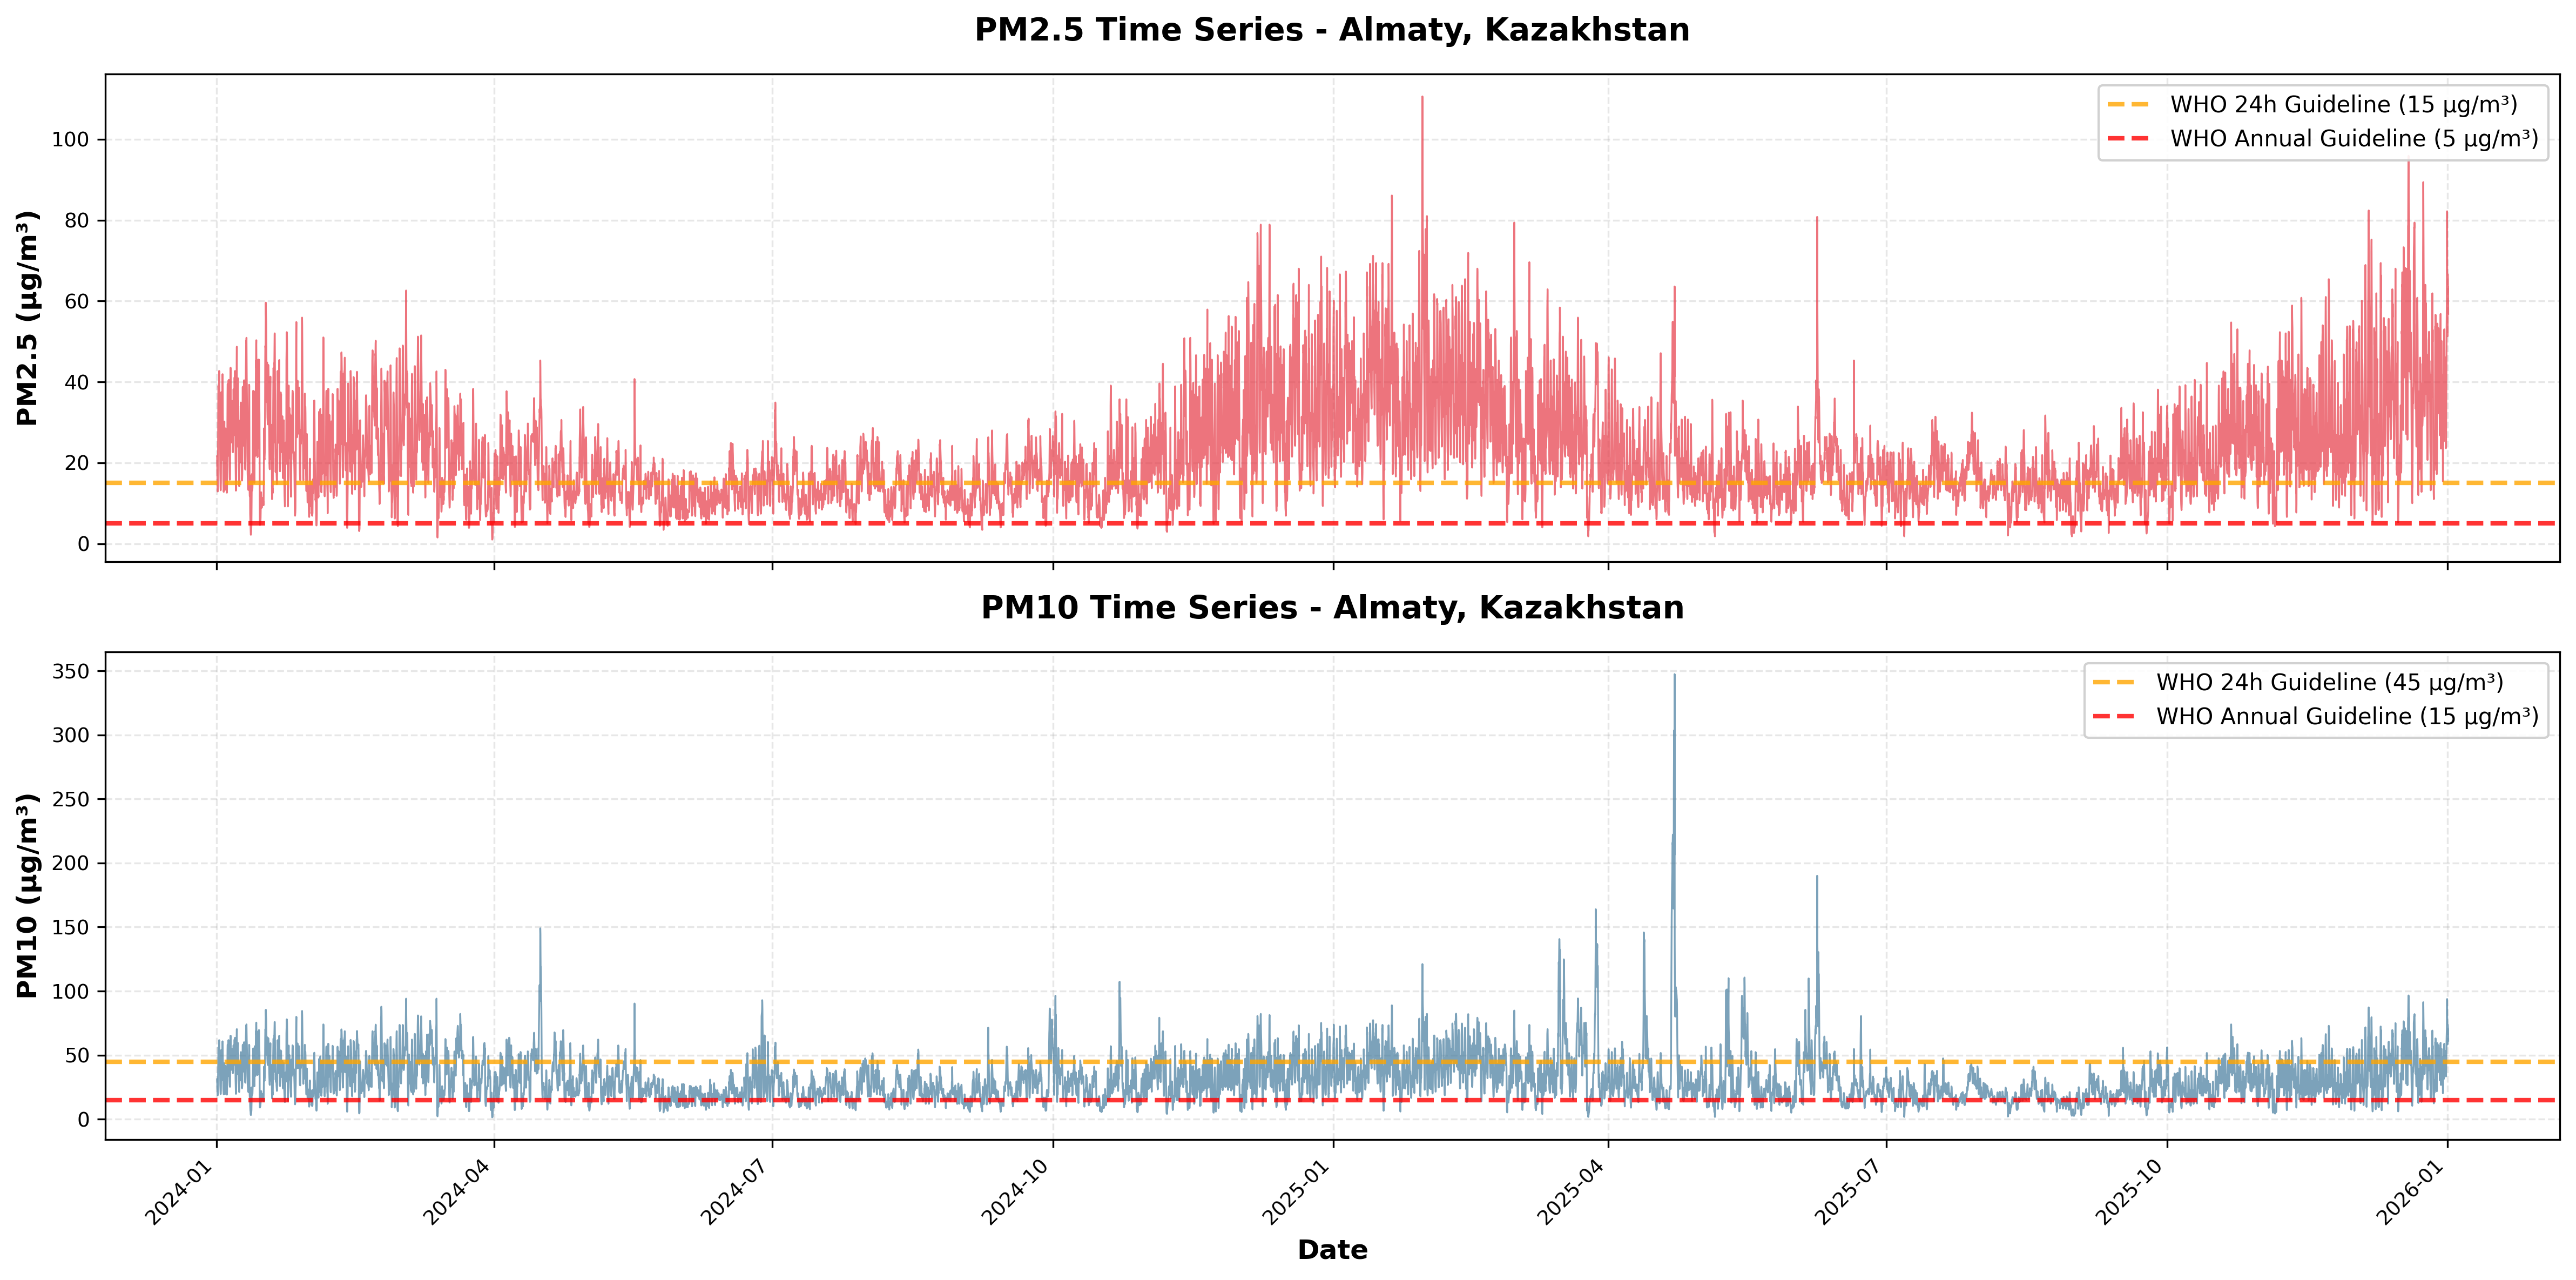
\includegraphics[width=0.95\textwidth]{time_series_full.png}
\caption{PM2.5 және PM10 толық уақыттық қатарлары (2024–2025)}
\label{fig:timeseries}
\end{figure}

\subsubsection{Үлестірім талдауы}

Сурет \ref{fig:distribution} PM2.5 және PM10 концентрацияларының үлестірімін көрсетеді. Екі айнымалы да оңға қисық (positive skewness) үлестірімге ие, яғни жоғары концентрациялар эпизодтық сипатта болады.

\begin{figure}[H]
\centering
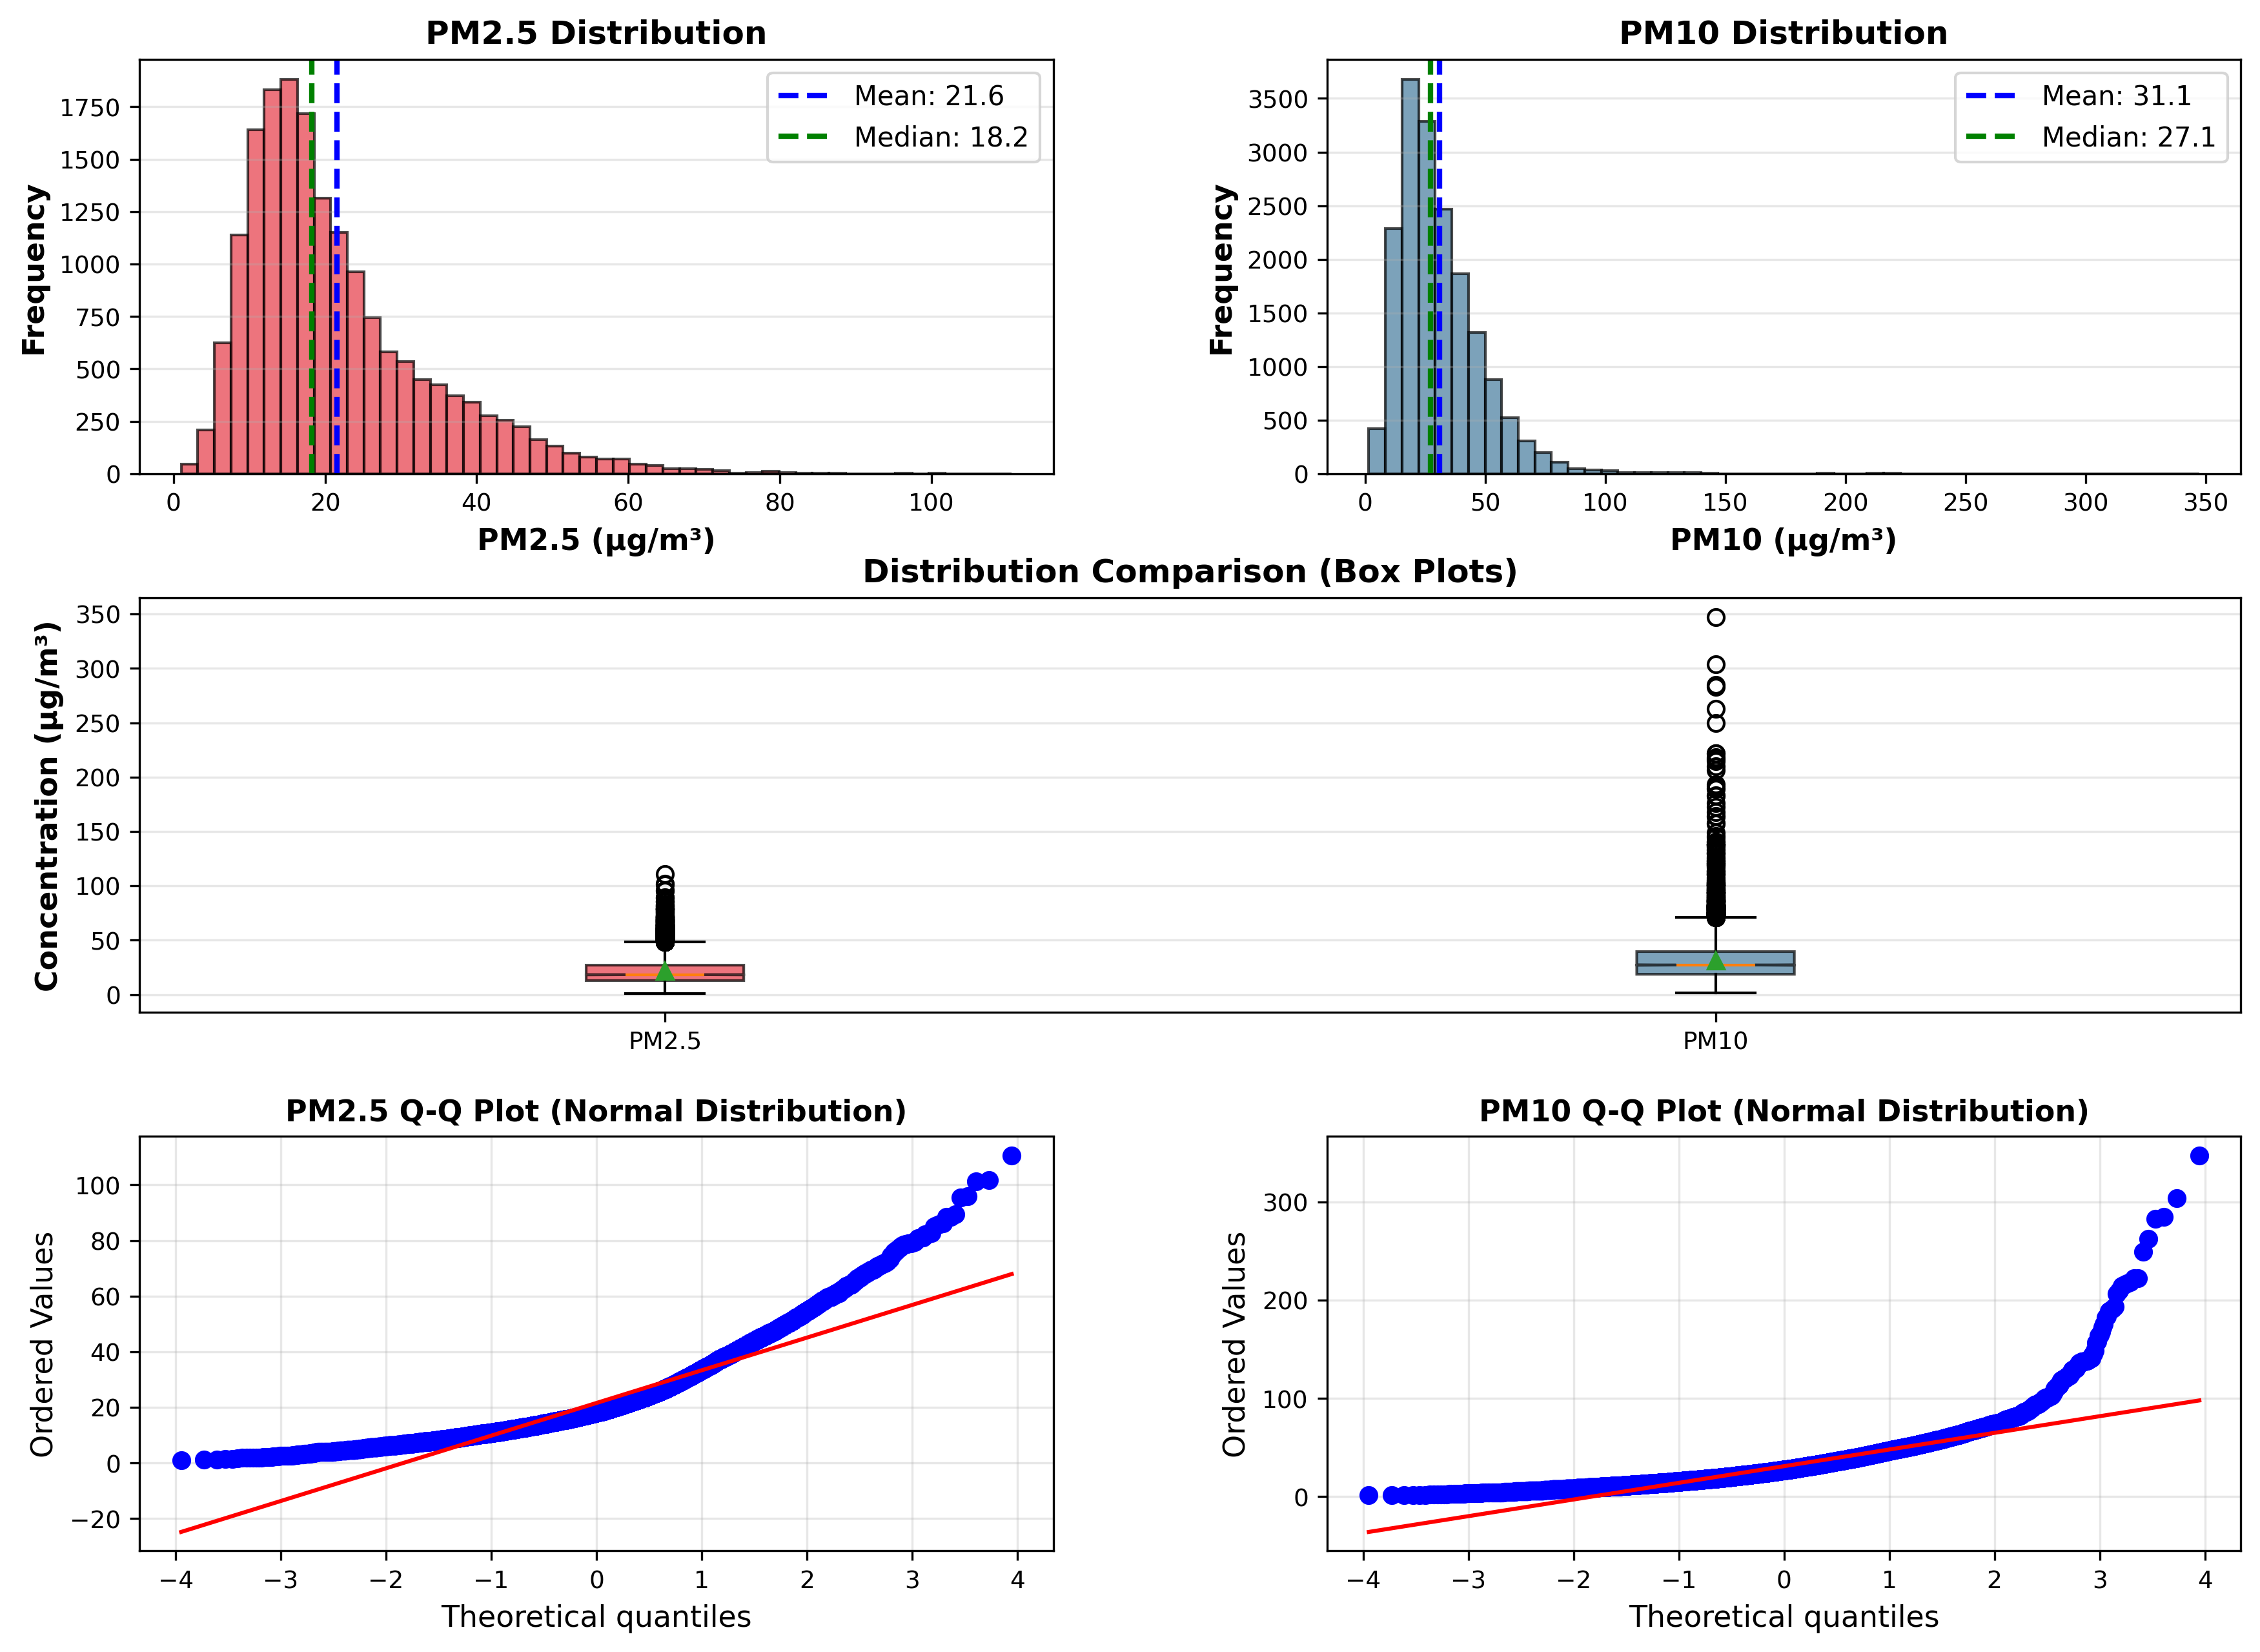
\includegraphics[width=0.9\textwidth]{distribution_analysis.png}
\caption{PM2.5 және PM10 үлестірімдері және қорытынды статистика}
\label{fig:distribution}
\end{figure}

\subsubsection{Корреляциялық талдау}

Сурет \ref{fig:correlation} PM2.5 және PM10 арасындағы корреляцияны көрсетеді. Екі айнымалы арасында жоғары оң корреляция байқалады (r > 0.8), бұл олардың ортақ көздері мен трансмиссия механизмдері бар екенін растайды.

\begin{figure}[htbp]
\centering
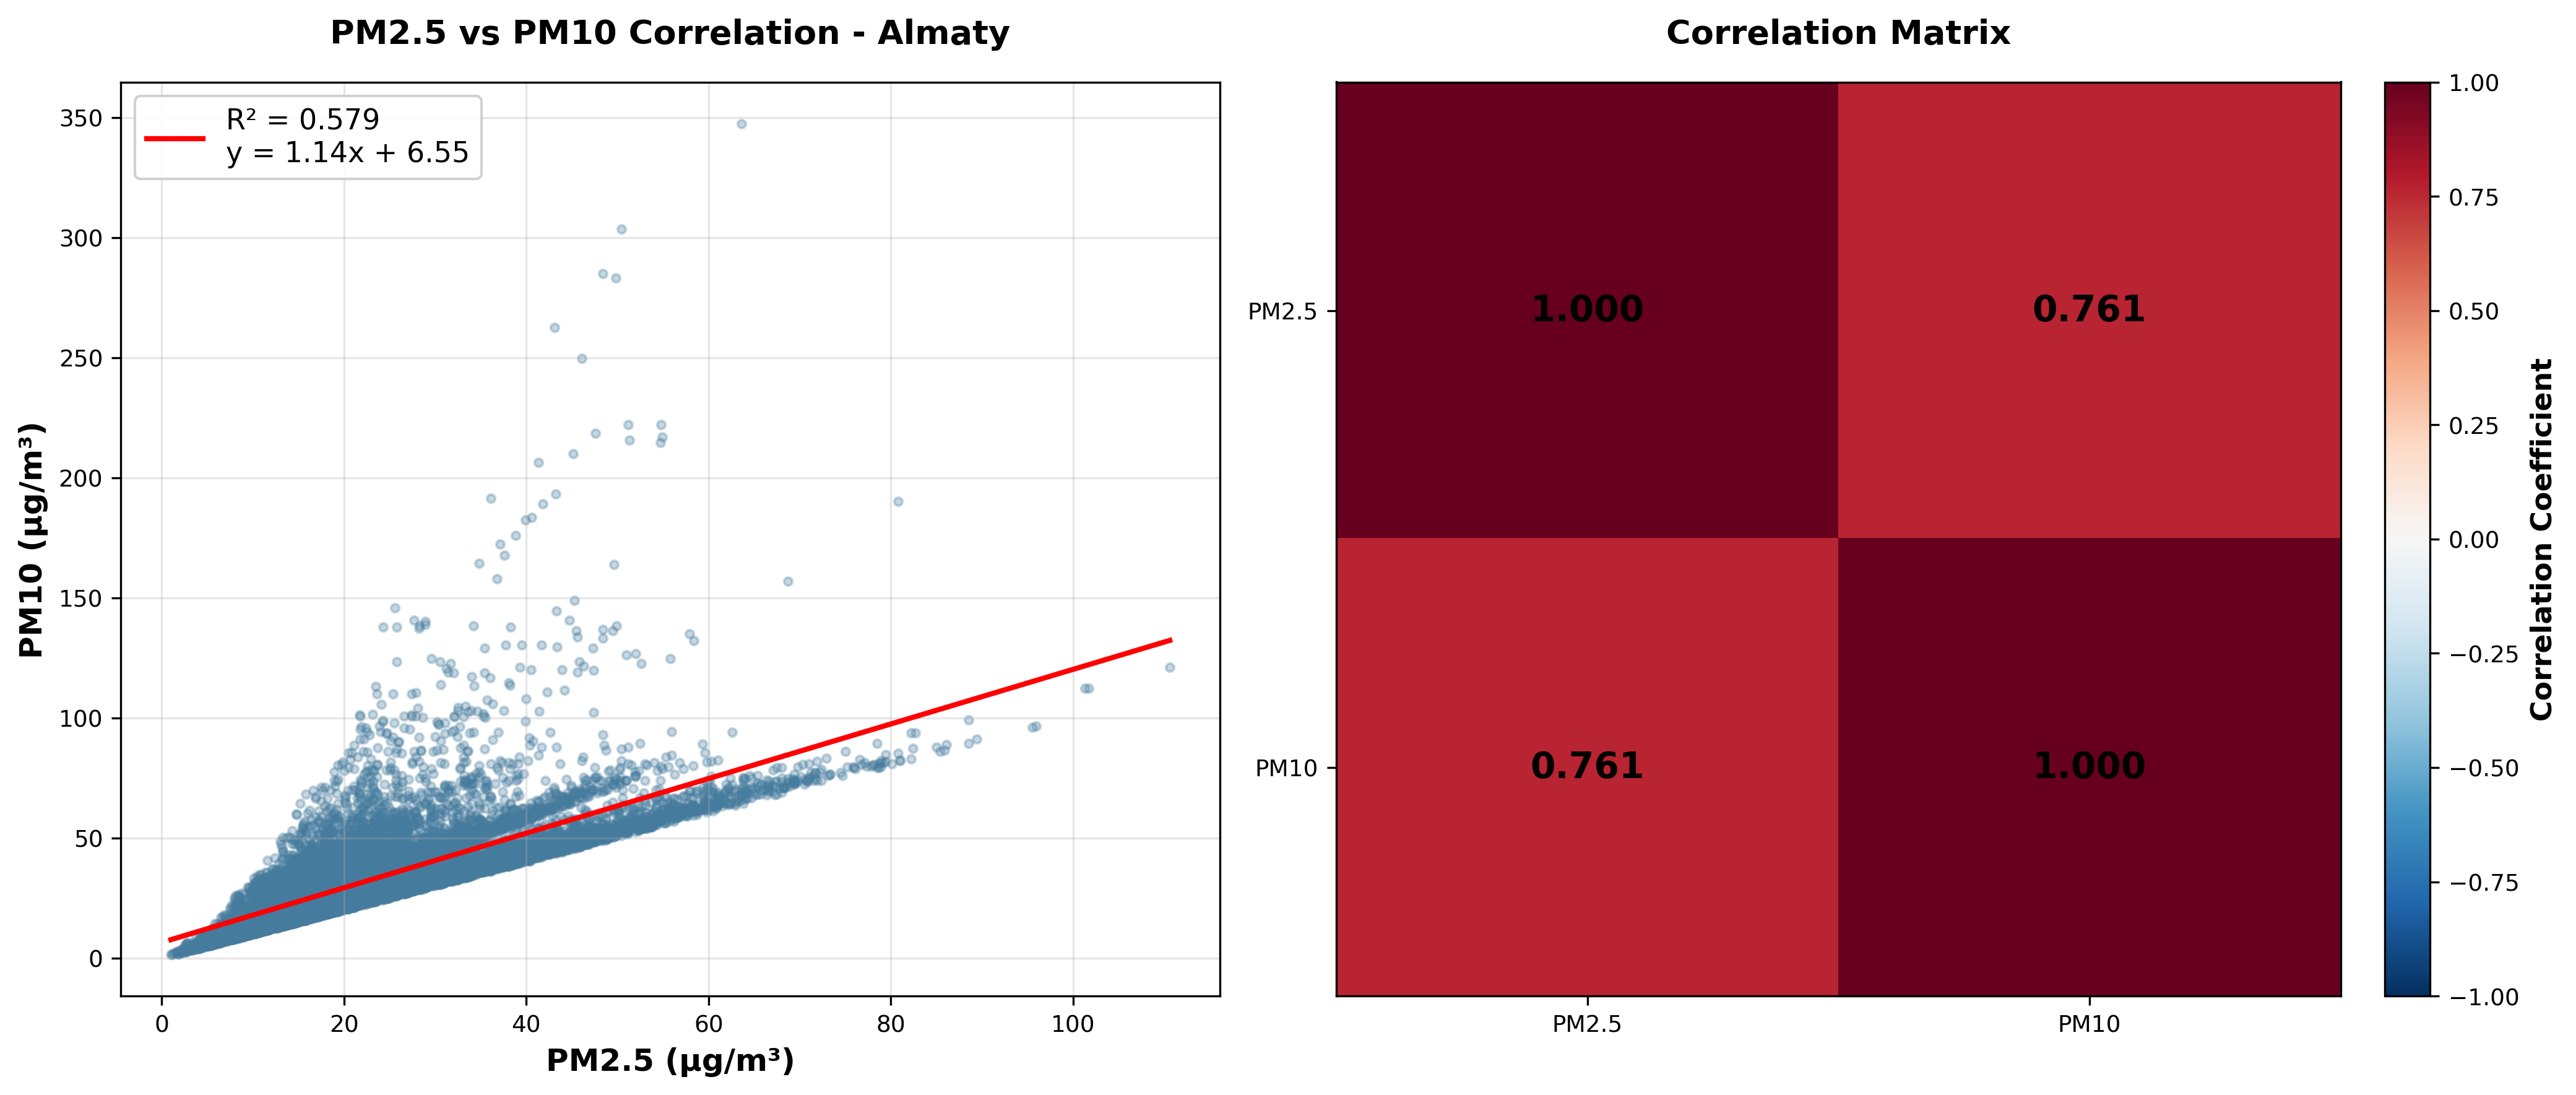
\includegraphics[width=0.9\textwidth]{correlation_analysis.png}
\caption{PM2.5 және PM10 корреляциялық талдау}
\label{fig:correlation}
\end{figure}

\subsubsection{Тәуліктік заңдылықтар}

Сурет \ref{fig:diurnal} PM2.5 және PM10 тәуліктік динамикасын көрсетеді. Екі шың байқалады: таңертеңгі (7–9 сағат) және кешкі (18–20 сағат). Бұл шыңдар көлік ағымдарының ұлғаюымен тікелей сәйкес келеді.

\begin{figure}[htbp]
\centering
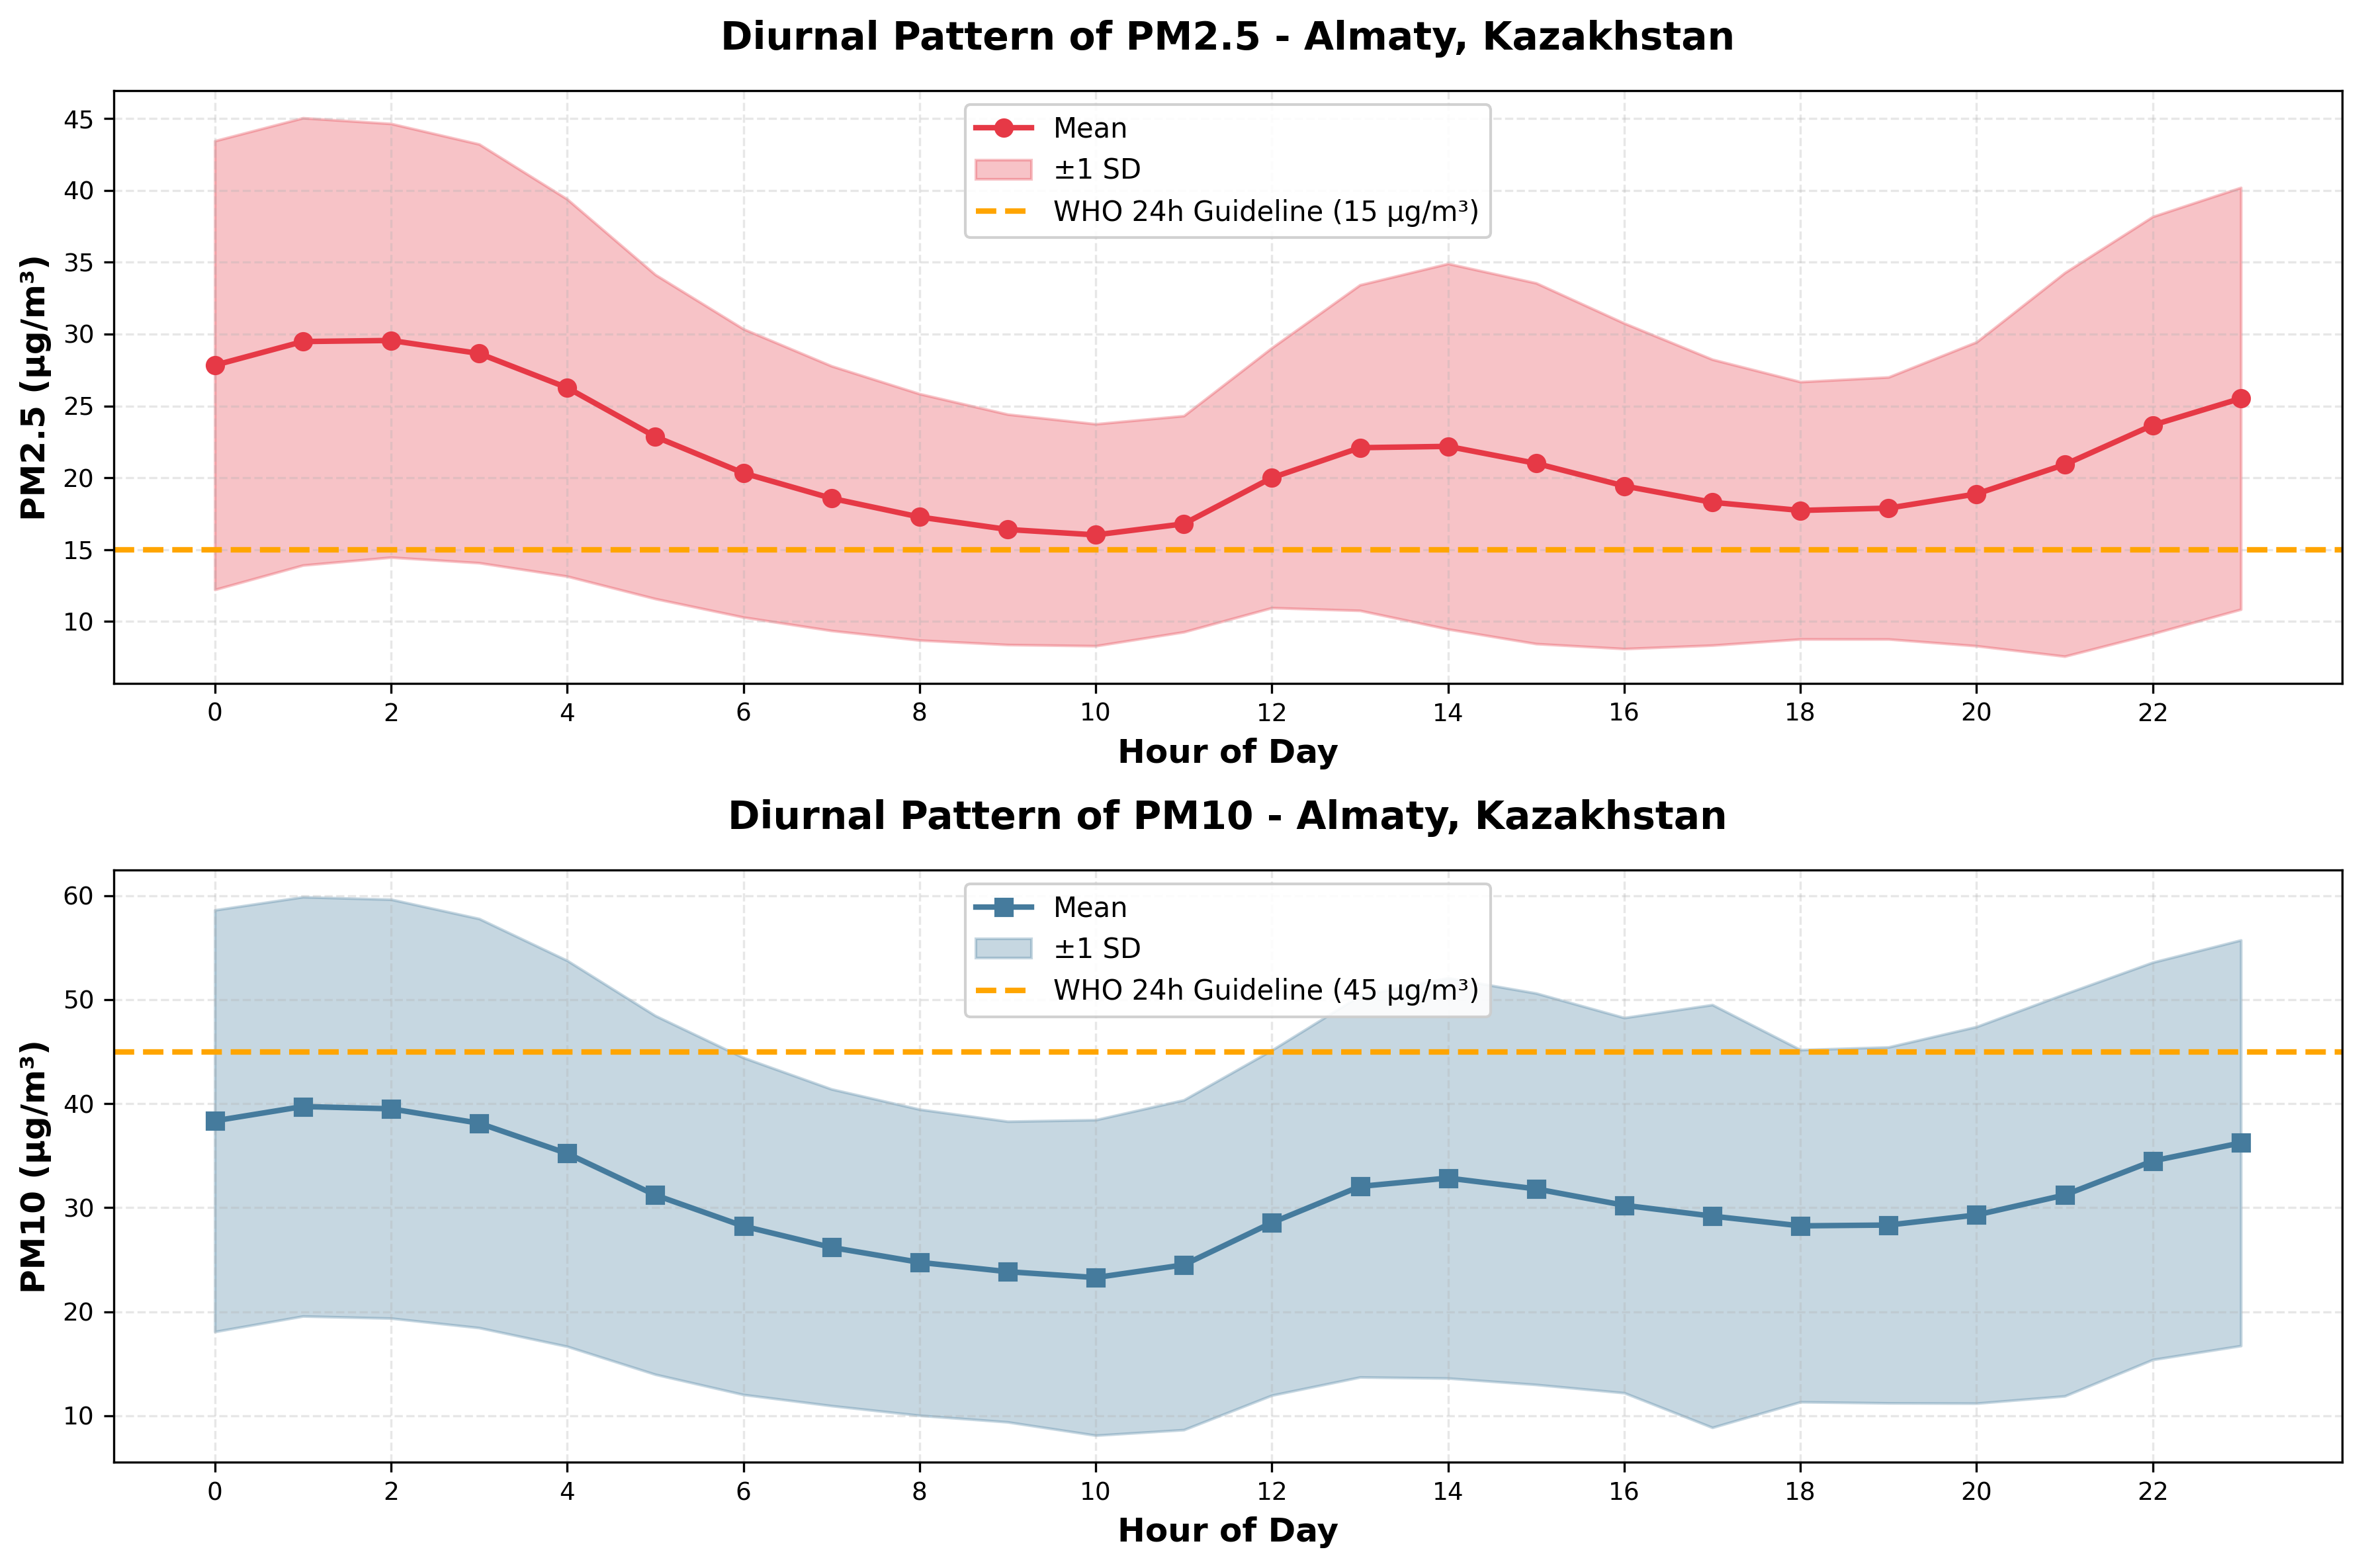
\includegraphics[width=0.9\textwidth]{diurnal_patterns.png}
\caption{PM2.5 және PM10 тәуліктік заңдылықтары}
\label{fig:diurnal}
\end{figure}

\subsubsection{Апталық заңдылықтар}

Сурет \ref{fig:weekly} апта күндері бойынша орташа концентрацияларды көрсетеді. Жұмыс күндері (дүйсенбі–жұма) концентрациялар демалыс күндеріне (сенбі–жексенбі) қарағанда жоғарырақ.

\begin{figure}[htbp]
\centering
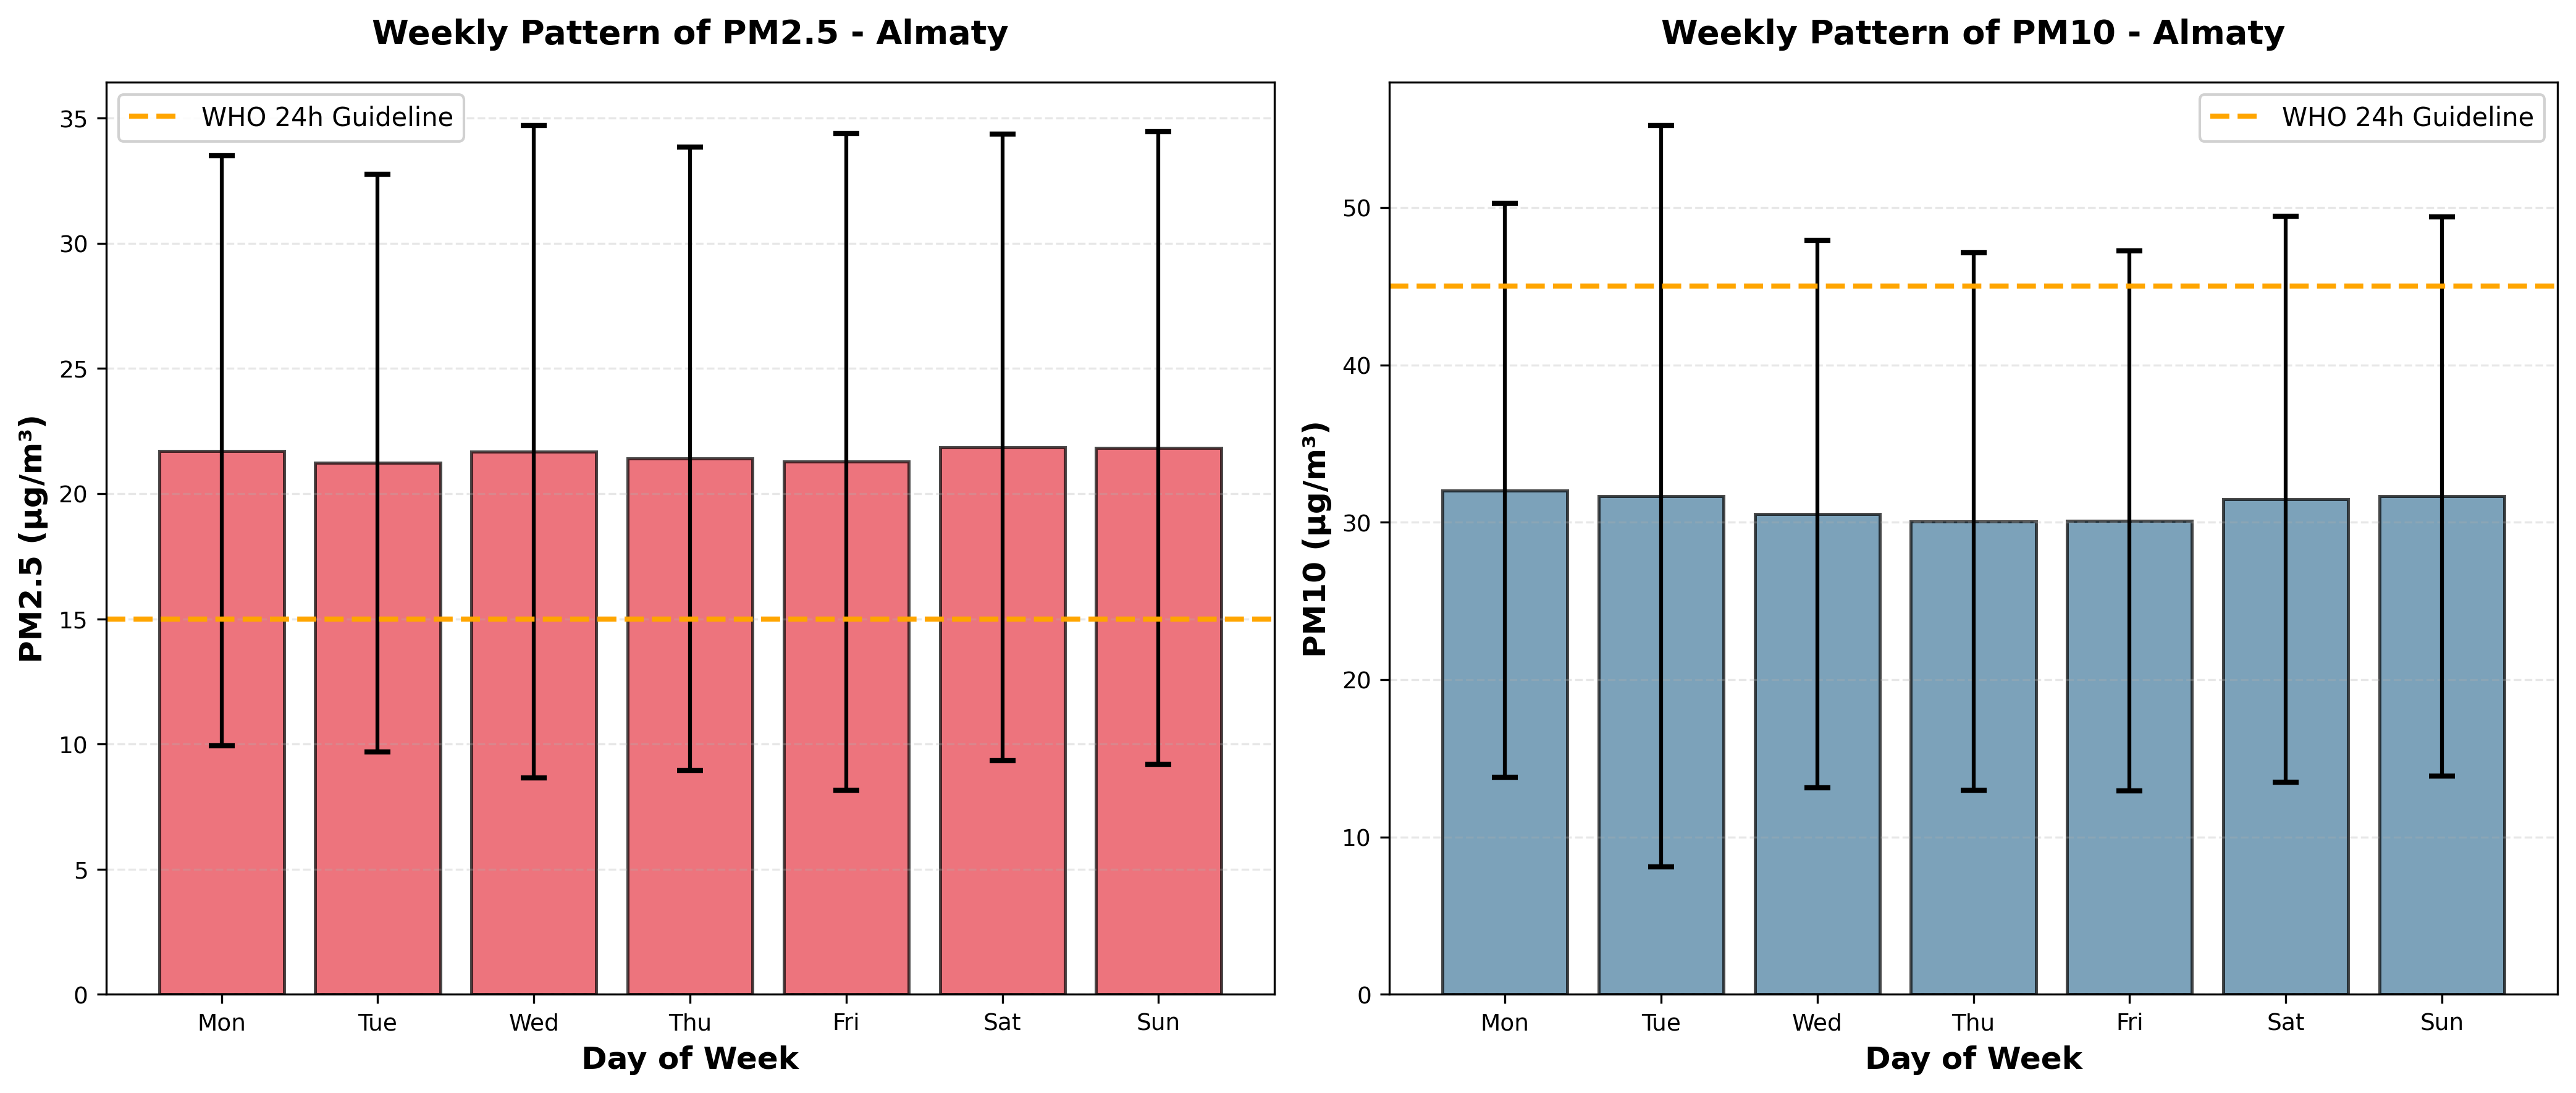
\includegraphics[width=0.9\textwidth]{weekly_patterns.png}
\caption{PM2.5 және PM10 апталық заңдылықтары}
\label{fig:weekly}
\end{figure}

\subsubsection{Маусымдық заңдылықтар}

Сурет \ref{fig:seasonal} маусымдық динамиканы көрсетеді. Қыс айларында концентрациялар 2–3 есе жоғарылайды, жаз айларында минимумға жетеді.

\begin{figure}[htbp]
\centering
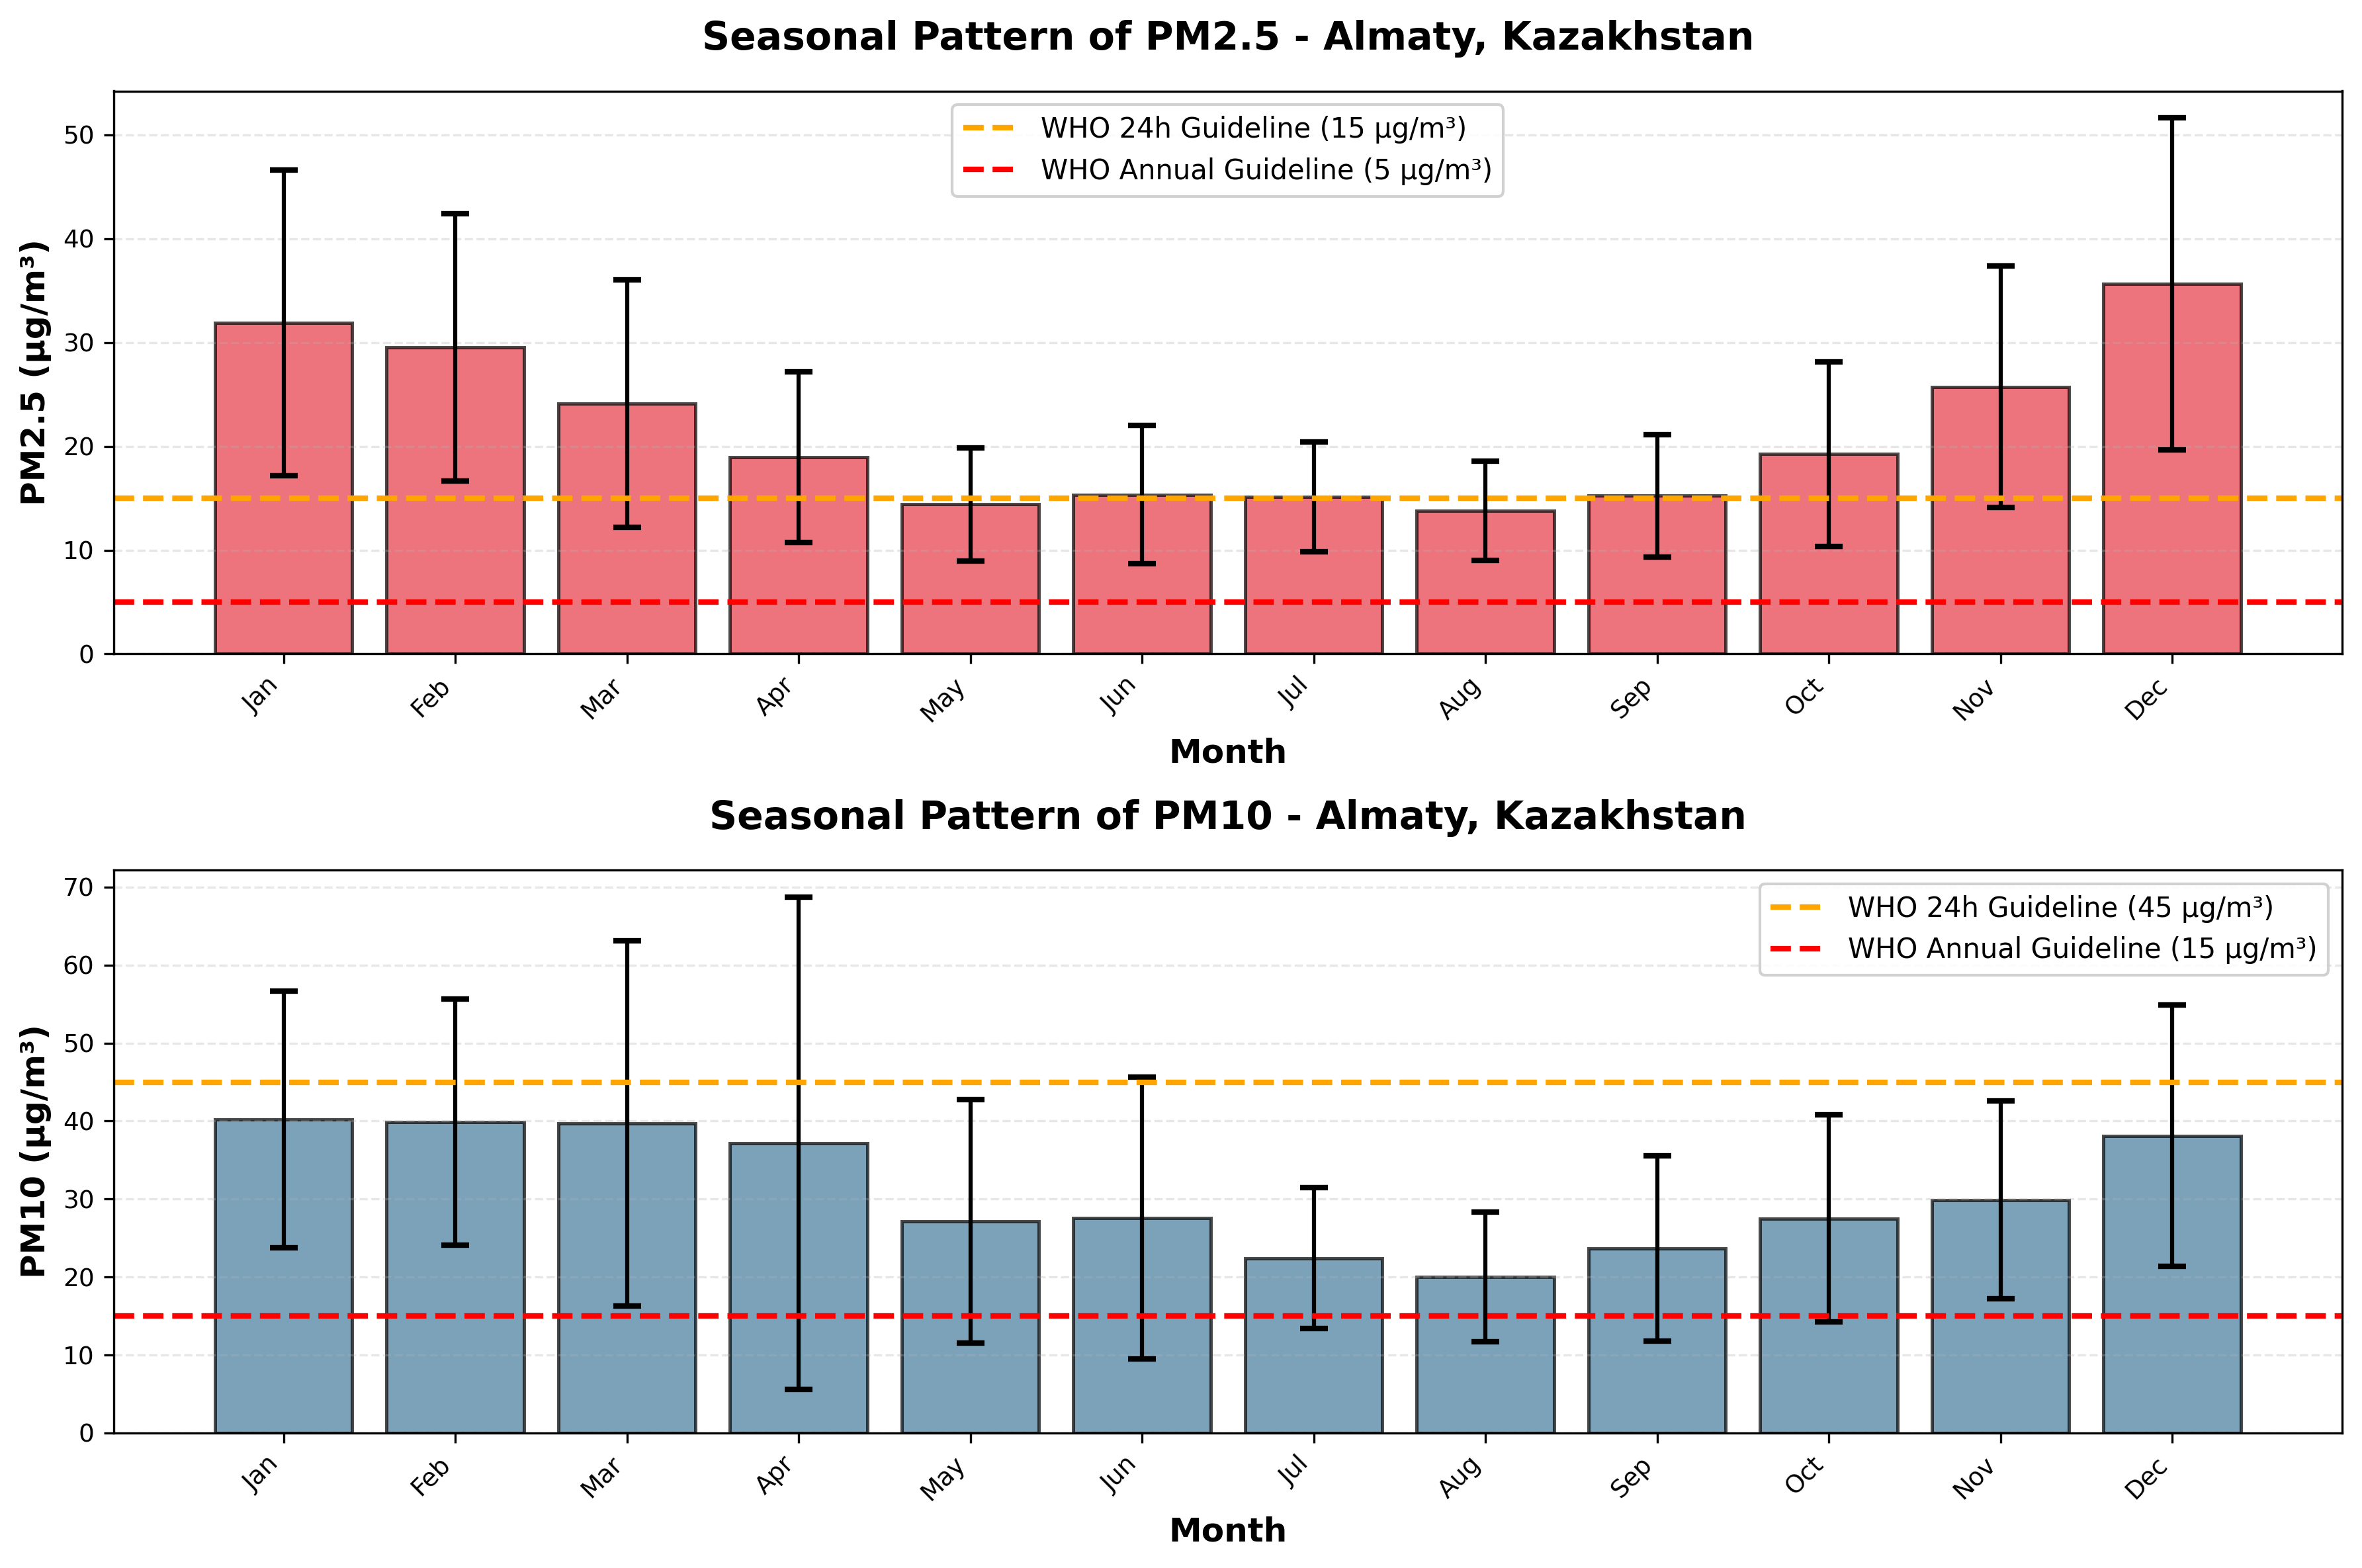
\includegraphics[width=0.9\textwidth]{seasonal_patterns.png}
\caption{PM2.5 және PM10 маусымдық заңдылықтары}
\label{fig:seasonal}
\end{figure}

\subsection{Модельдеу нәтижелері}

\subsubsection{PM2.5 болжамдары}

Сурет \ref{fig:pm25comparison} PM2.5 үшін барлық модельдердің салыстырмалы өнімділігін көрсетеді. Gradient Boosting моделі барлық метрикалар бойынша басымдық көрсетеді \cite{friedman2001}.

\begin{figure}[H]
\centering
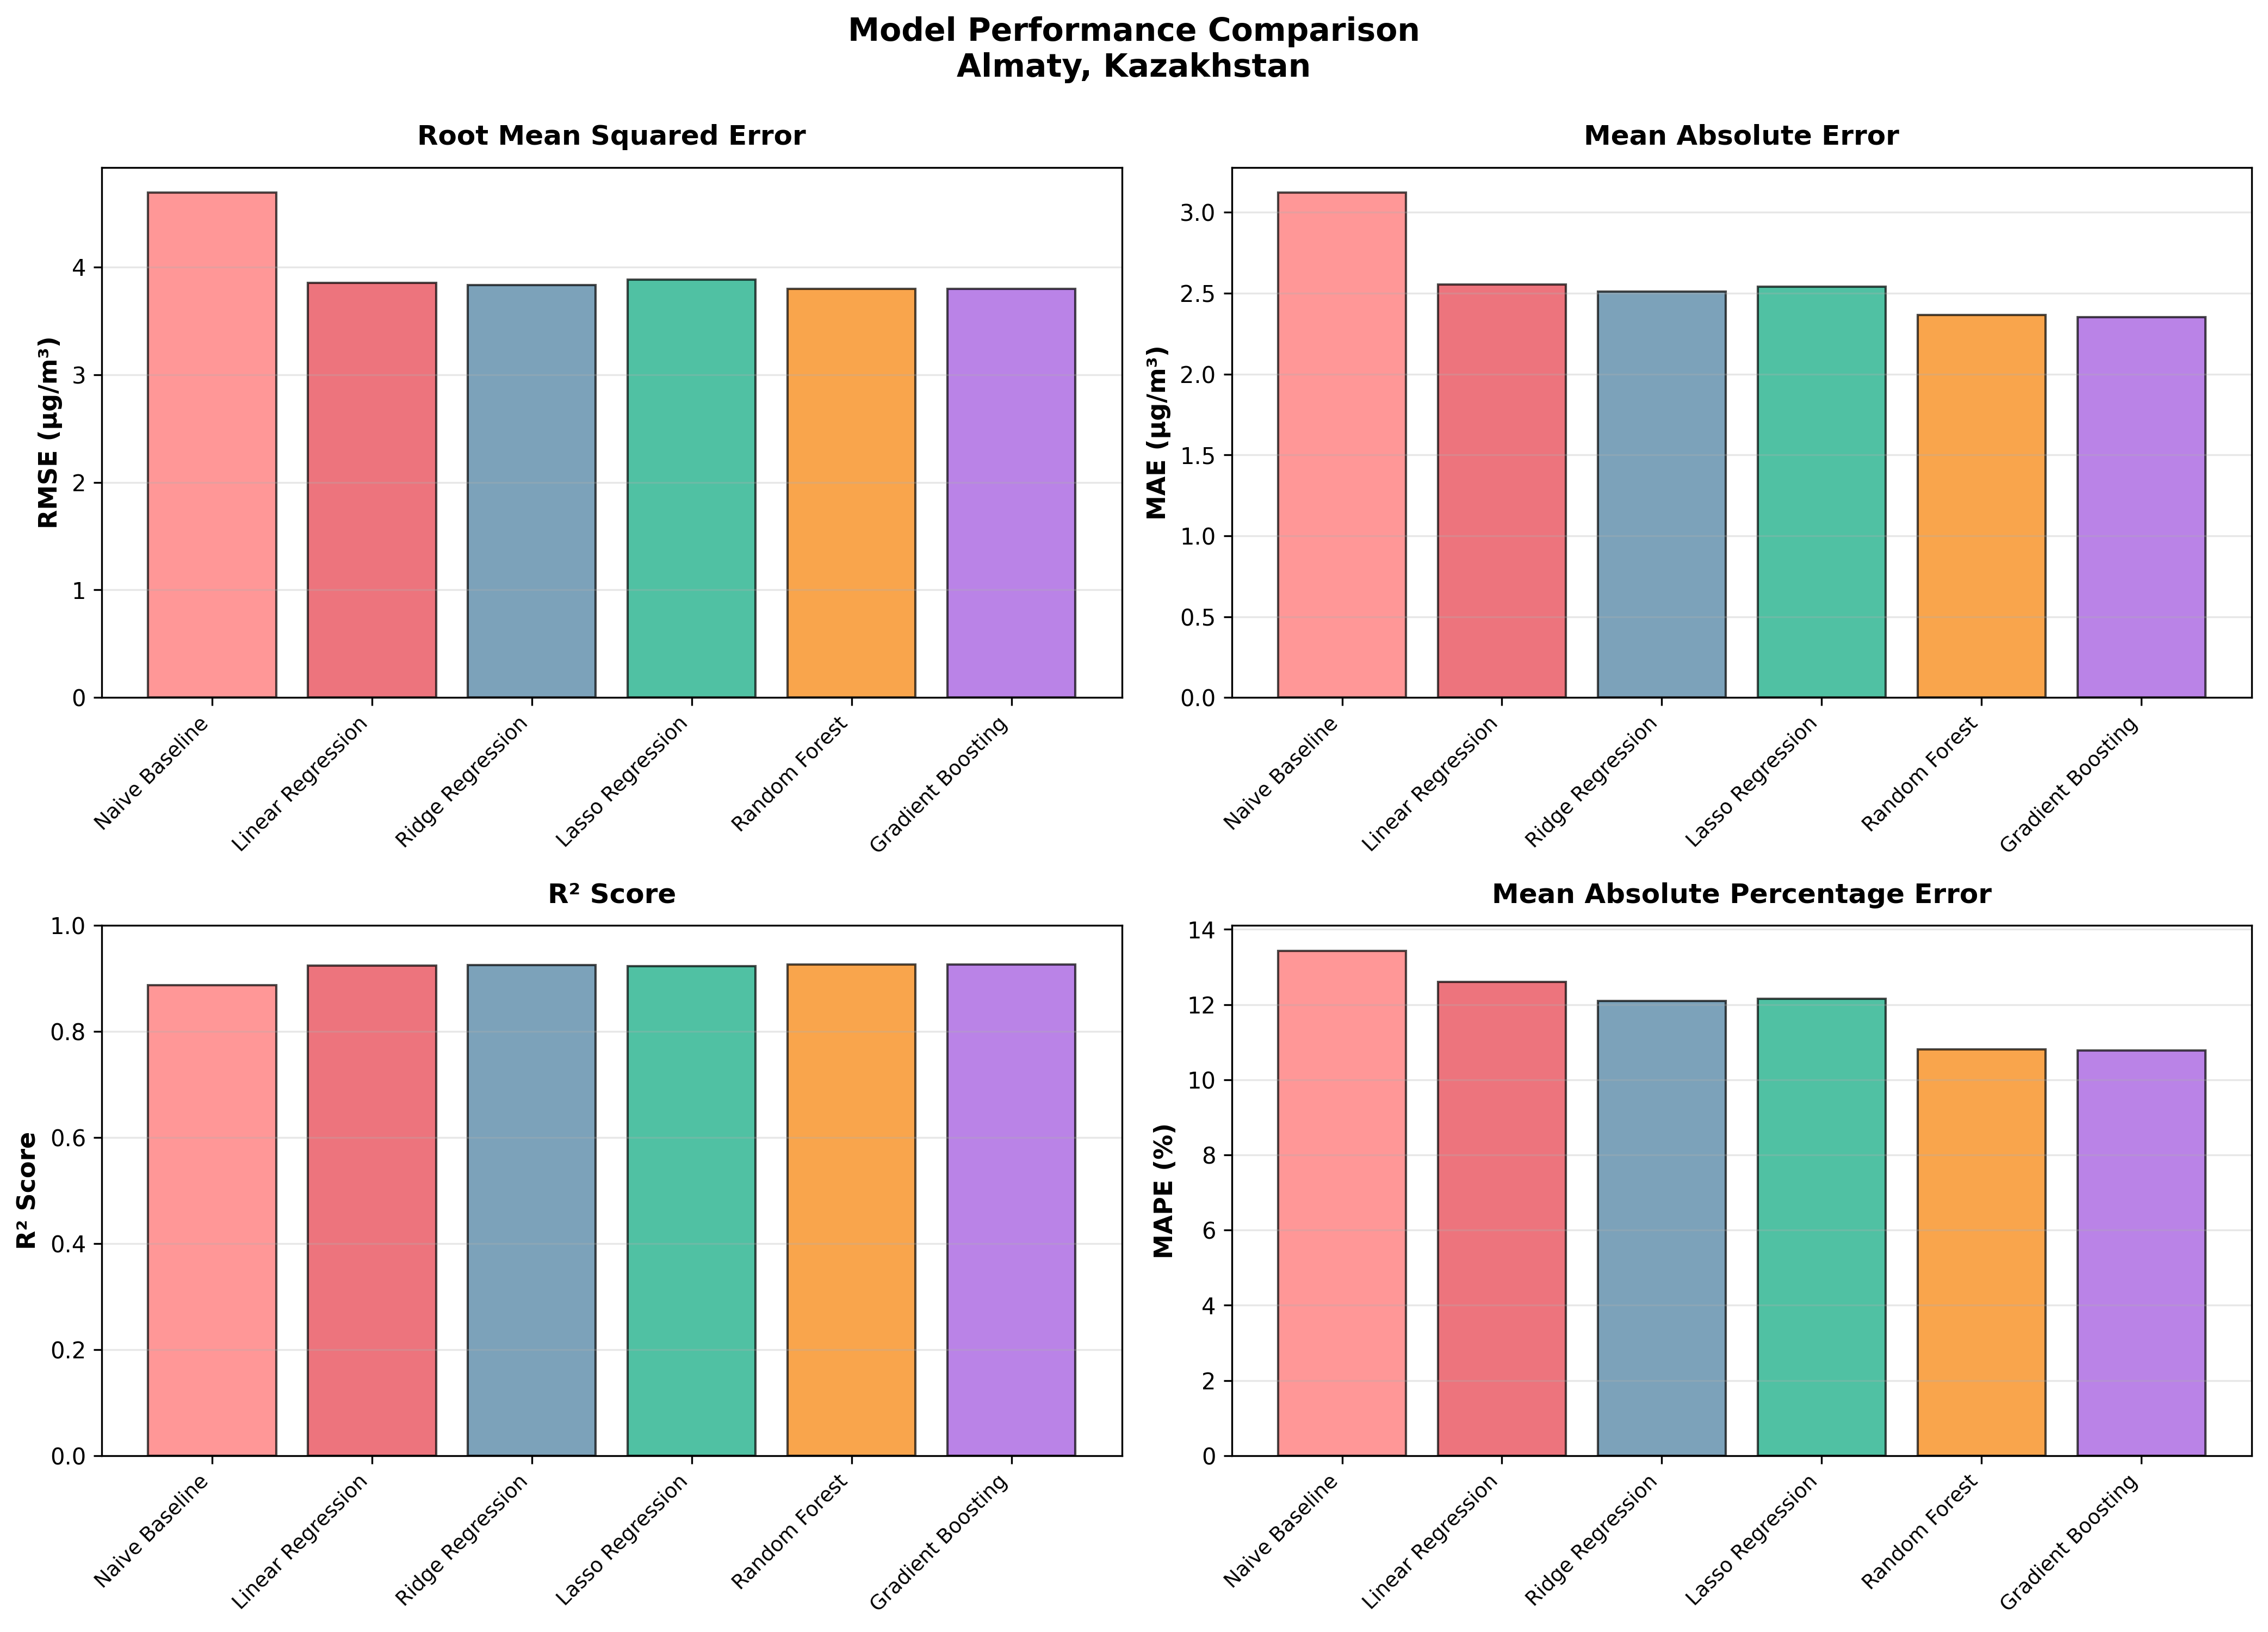
\includegraphics[width=0.9\textwidth]{model_comparison_pm25_t1.png}
\caption{PM2.5 модельдерінің салыстырмасы (RMSE, MAE, R², MAPE)}
\label{fig:pm25comparison}
\end{figure}

Сурет \ref{fig:pm25predictions} Gradient Boosting моделінің PM2.5 болжамдары мен нақты мәндерді көрсетеді. Модель уақыттық динамиканы жақсы ұстайды және шыңдар мен ойпаттарды дәл болжайды.

\begin{figure}[htbp]
\centering
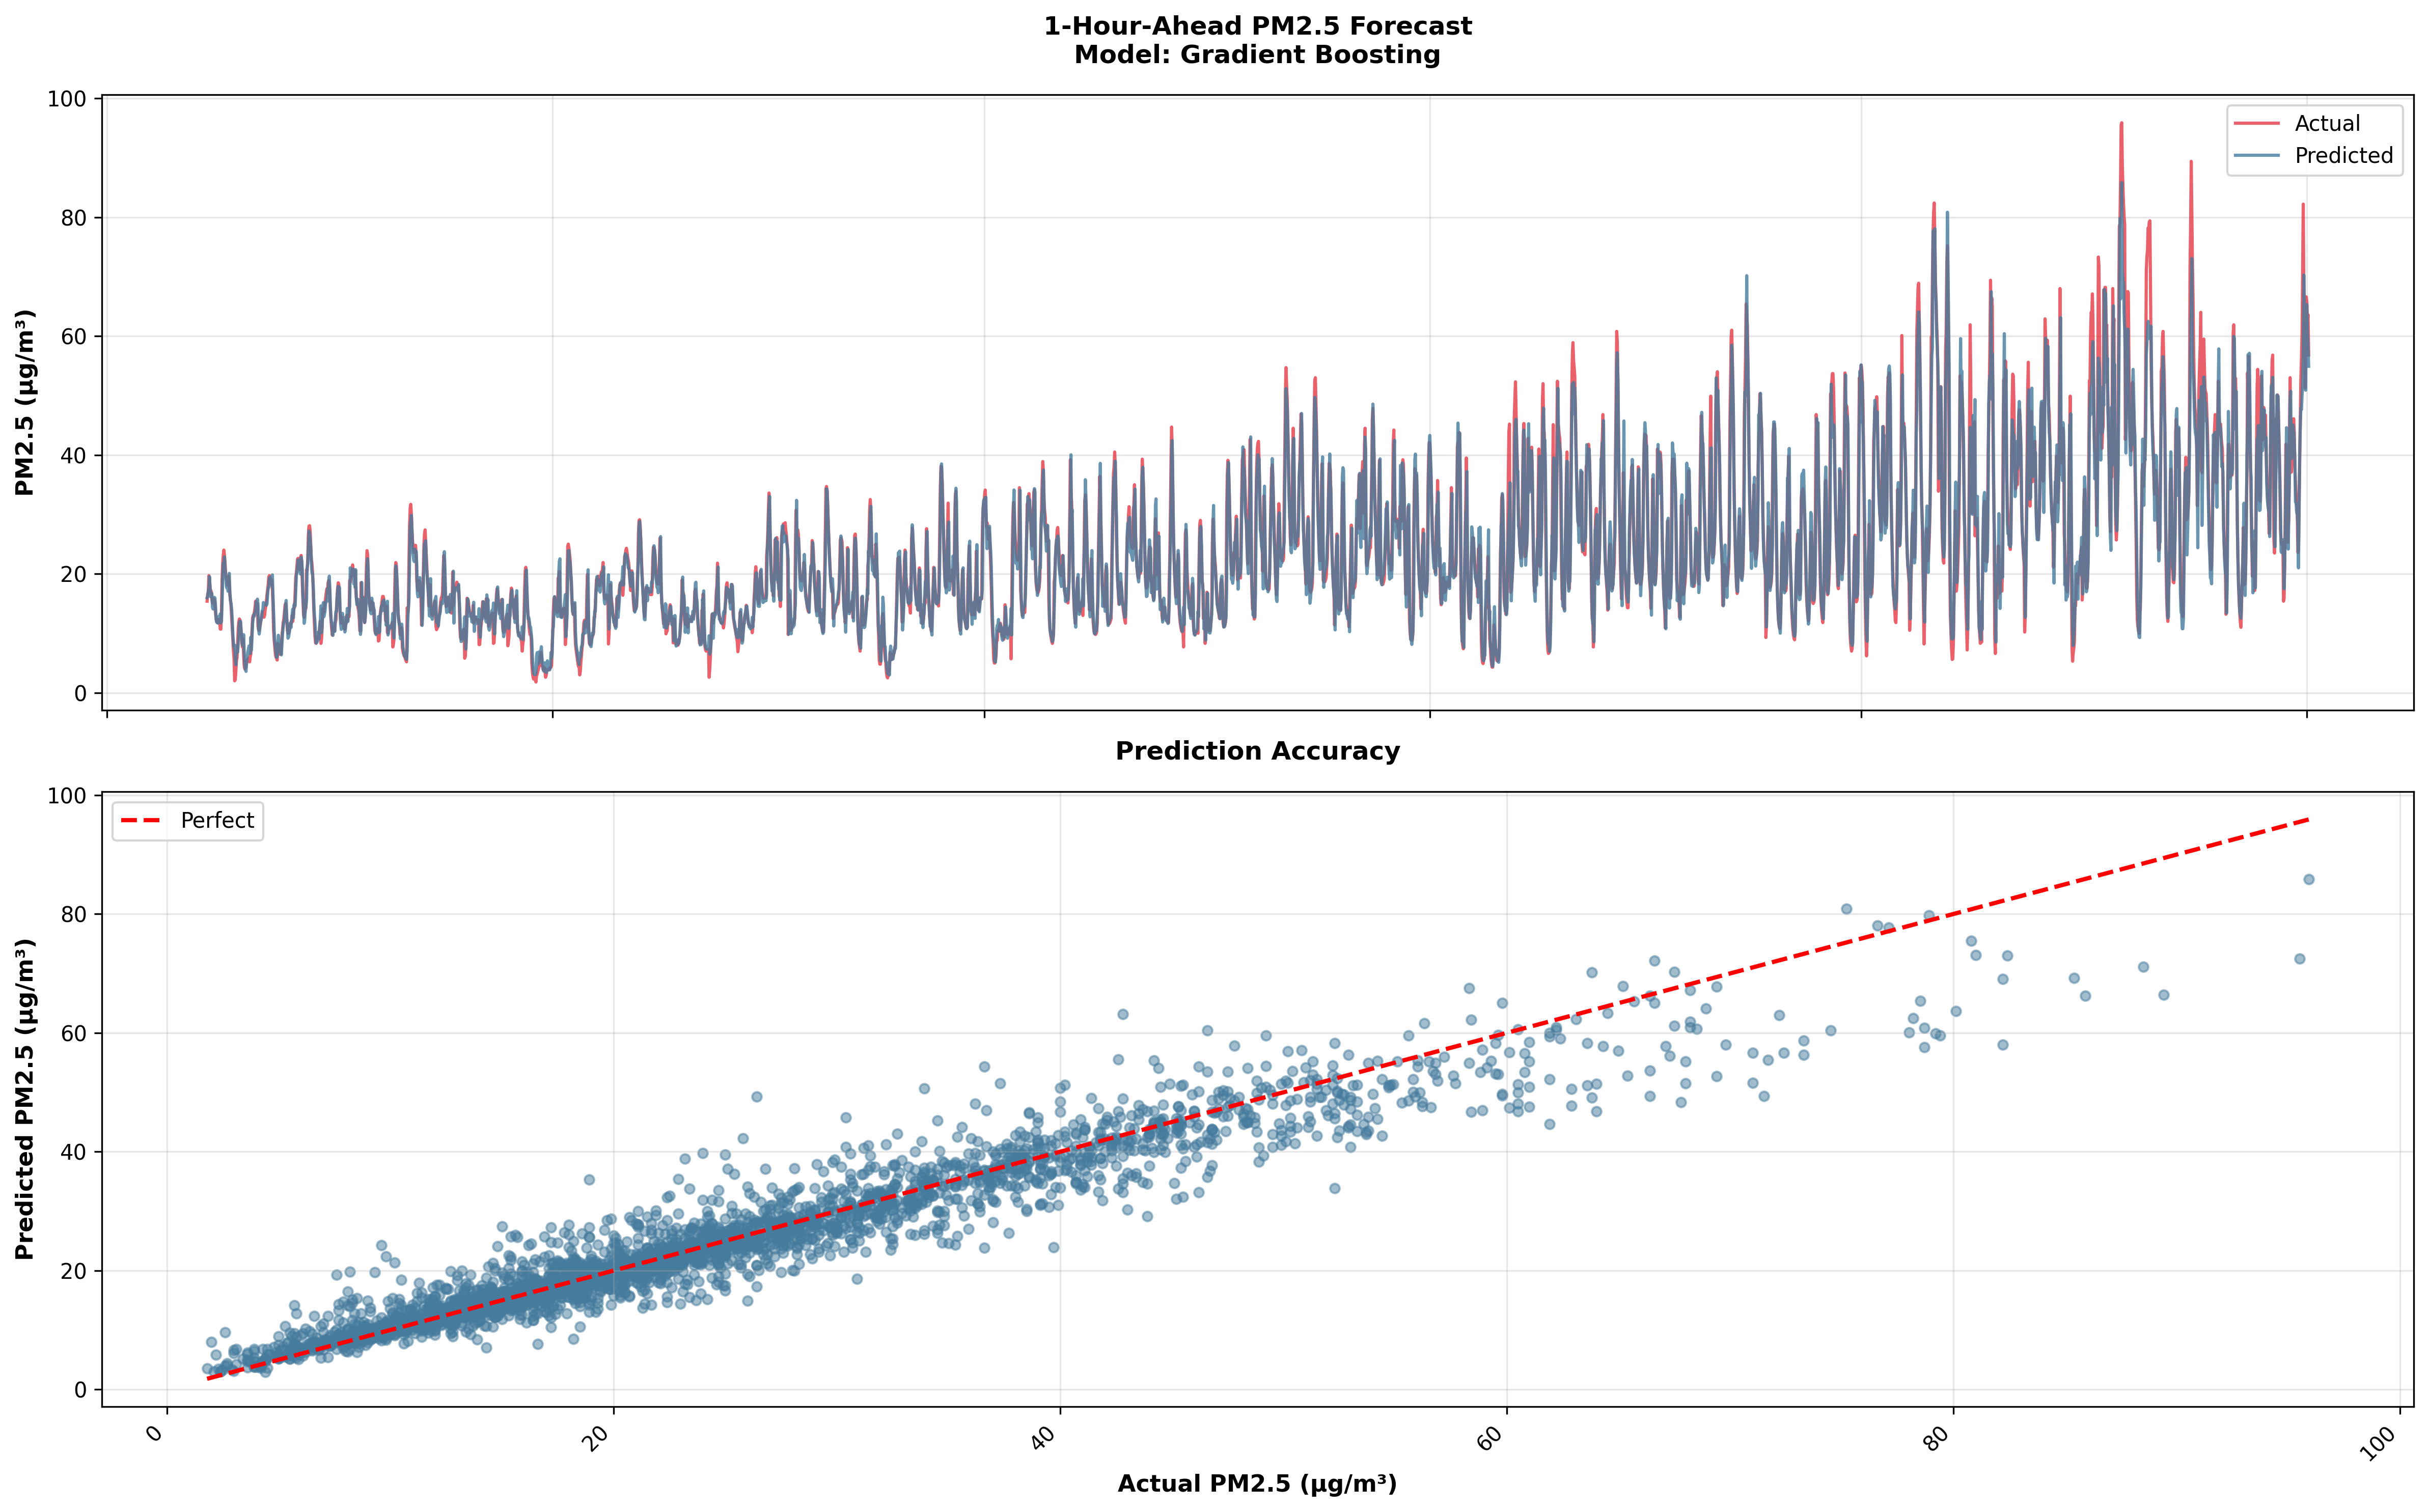
\includegraphics[width=0.95\textwidth]{predictions_vs_actual_pm25_t1.png}
\caption{PM2.5 болжамдары мен нақты мәндер (Gradient Boosting)}
\label{fig:pm25predictions}
\end{figure}

Сурет \ref{fig:pm25residuals} PM2.5 үшін residual (қалдық) талдауын көрсетеді. Residual-дар шамамен нормалды үлестірімге жақын және нөлдік орташа мән айналасында орналасқан.

\begin{figure}[htbp]
\centering
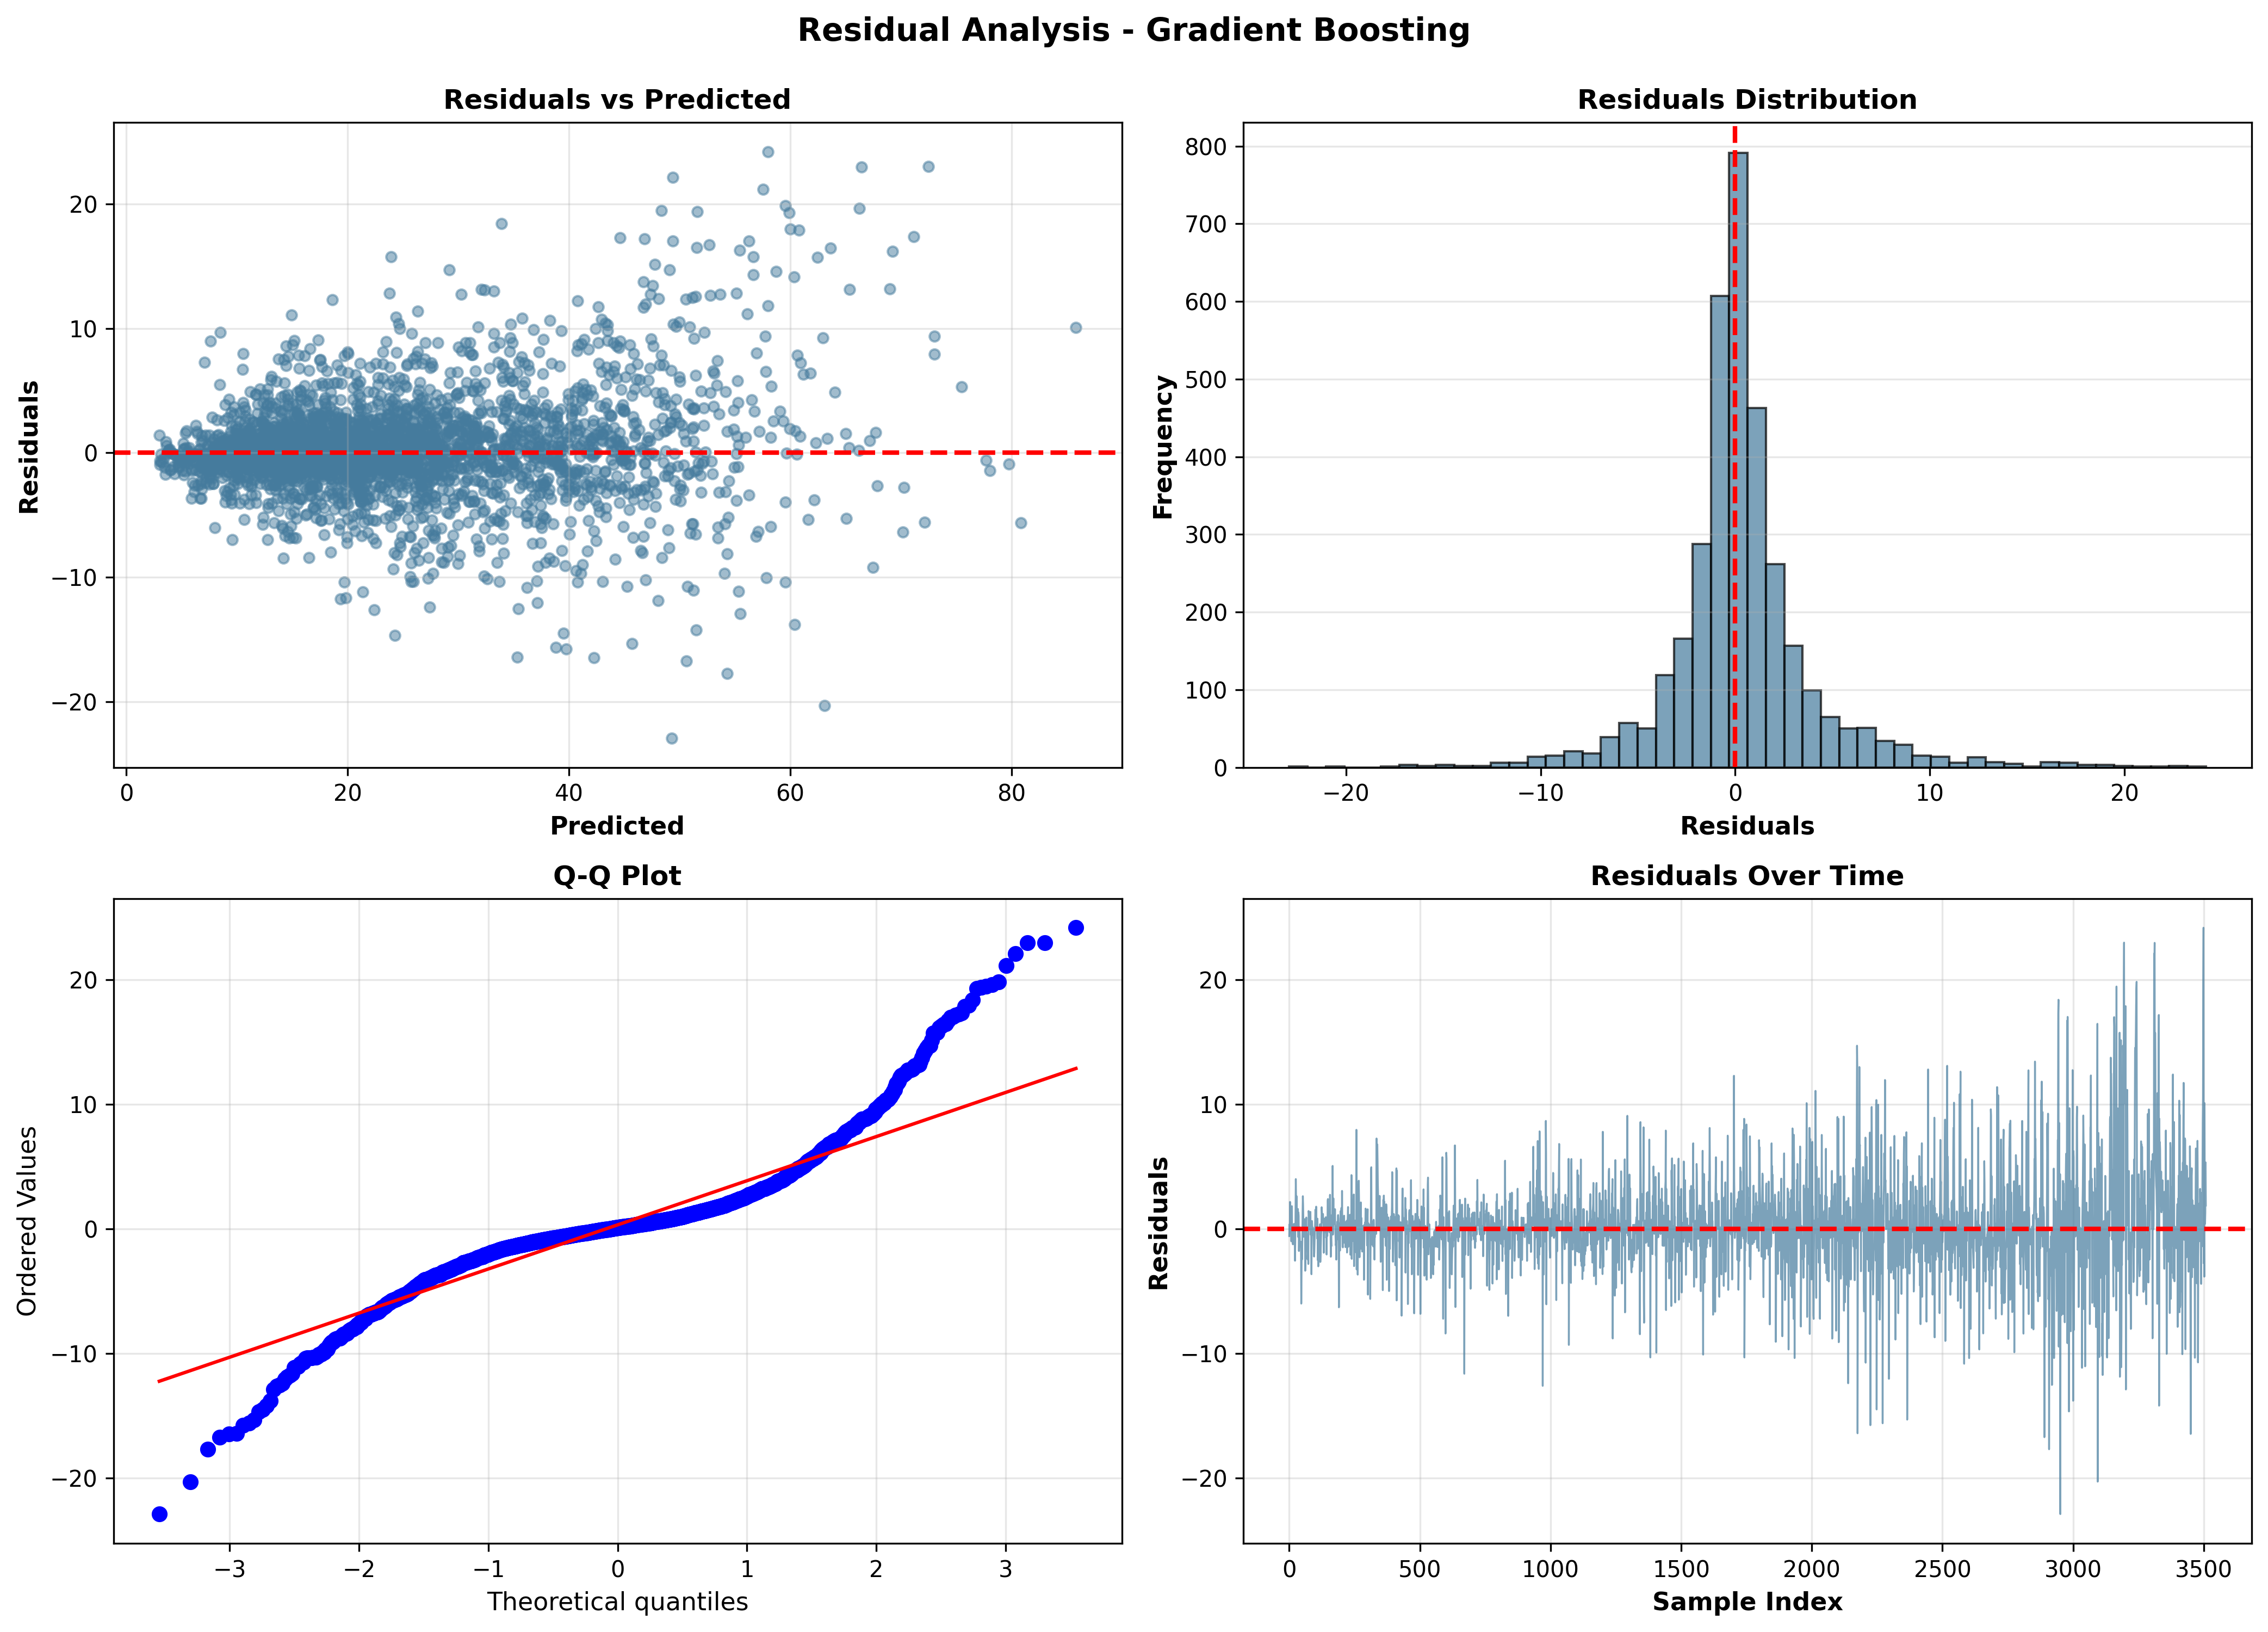
\includegraphics[width=0.95\textwidth]{residual_analysis_pm25_t1.png}
\caption{PM2.5 residual талдау (Gradient Boosting)}
\label{fig:pm25residuals}
\end{figure}

Сурет \ref{fig:pm25features} PM2.5 үшін белгілердің маңыздылығын көрсетеді \cite{breiman2001,molnar2020}. pm25\_lag\_1 (1 сағат бұрынғы мән) ең маңызды белгі болып табылады.

\begin{figure}[htbp]
\centering
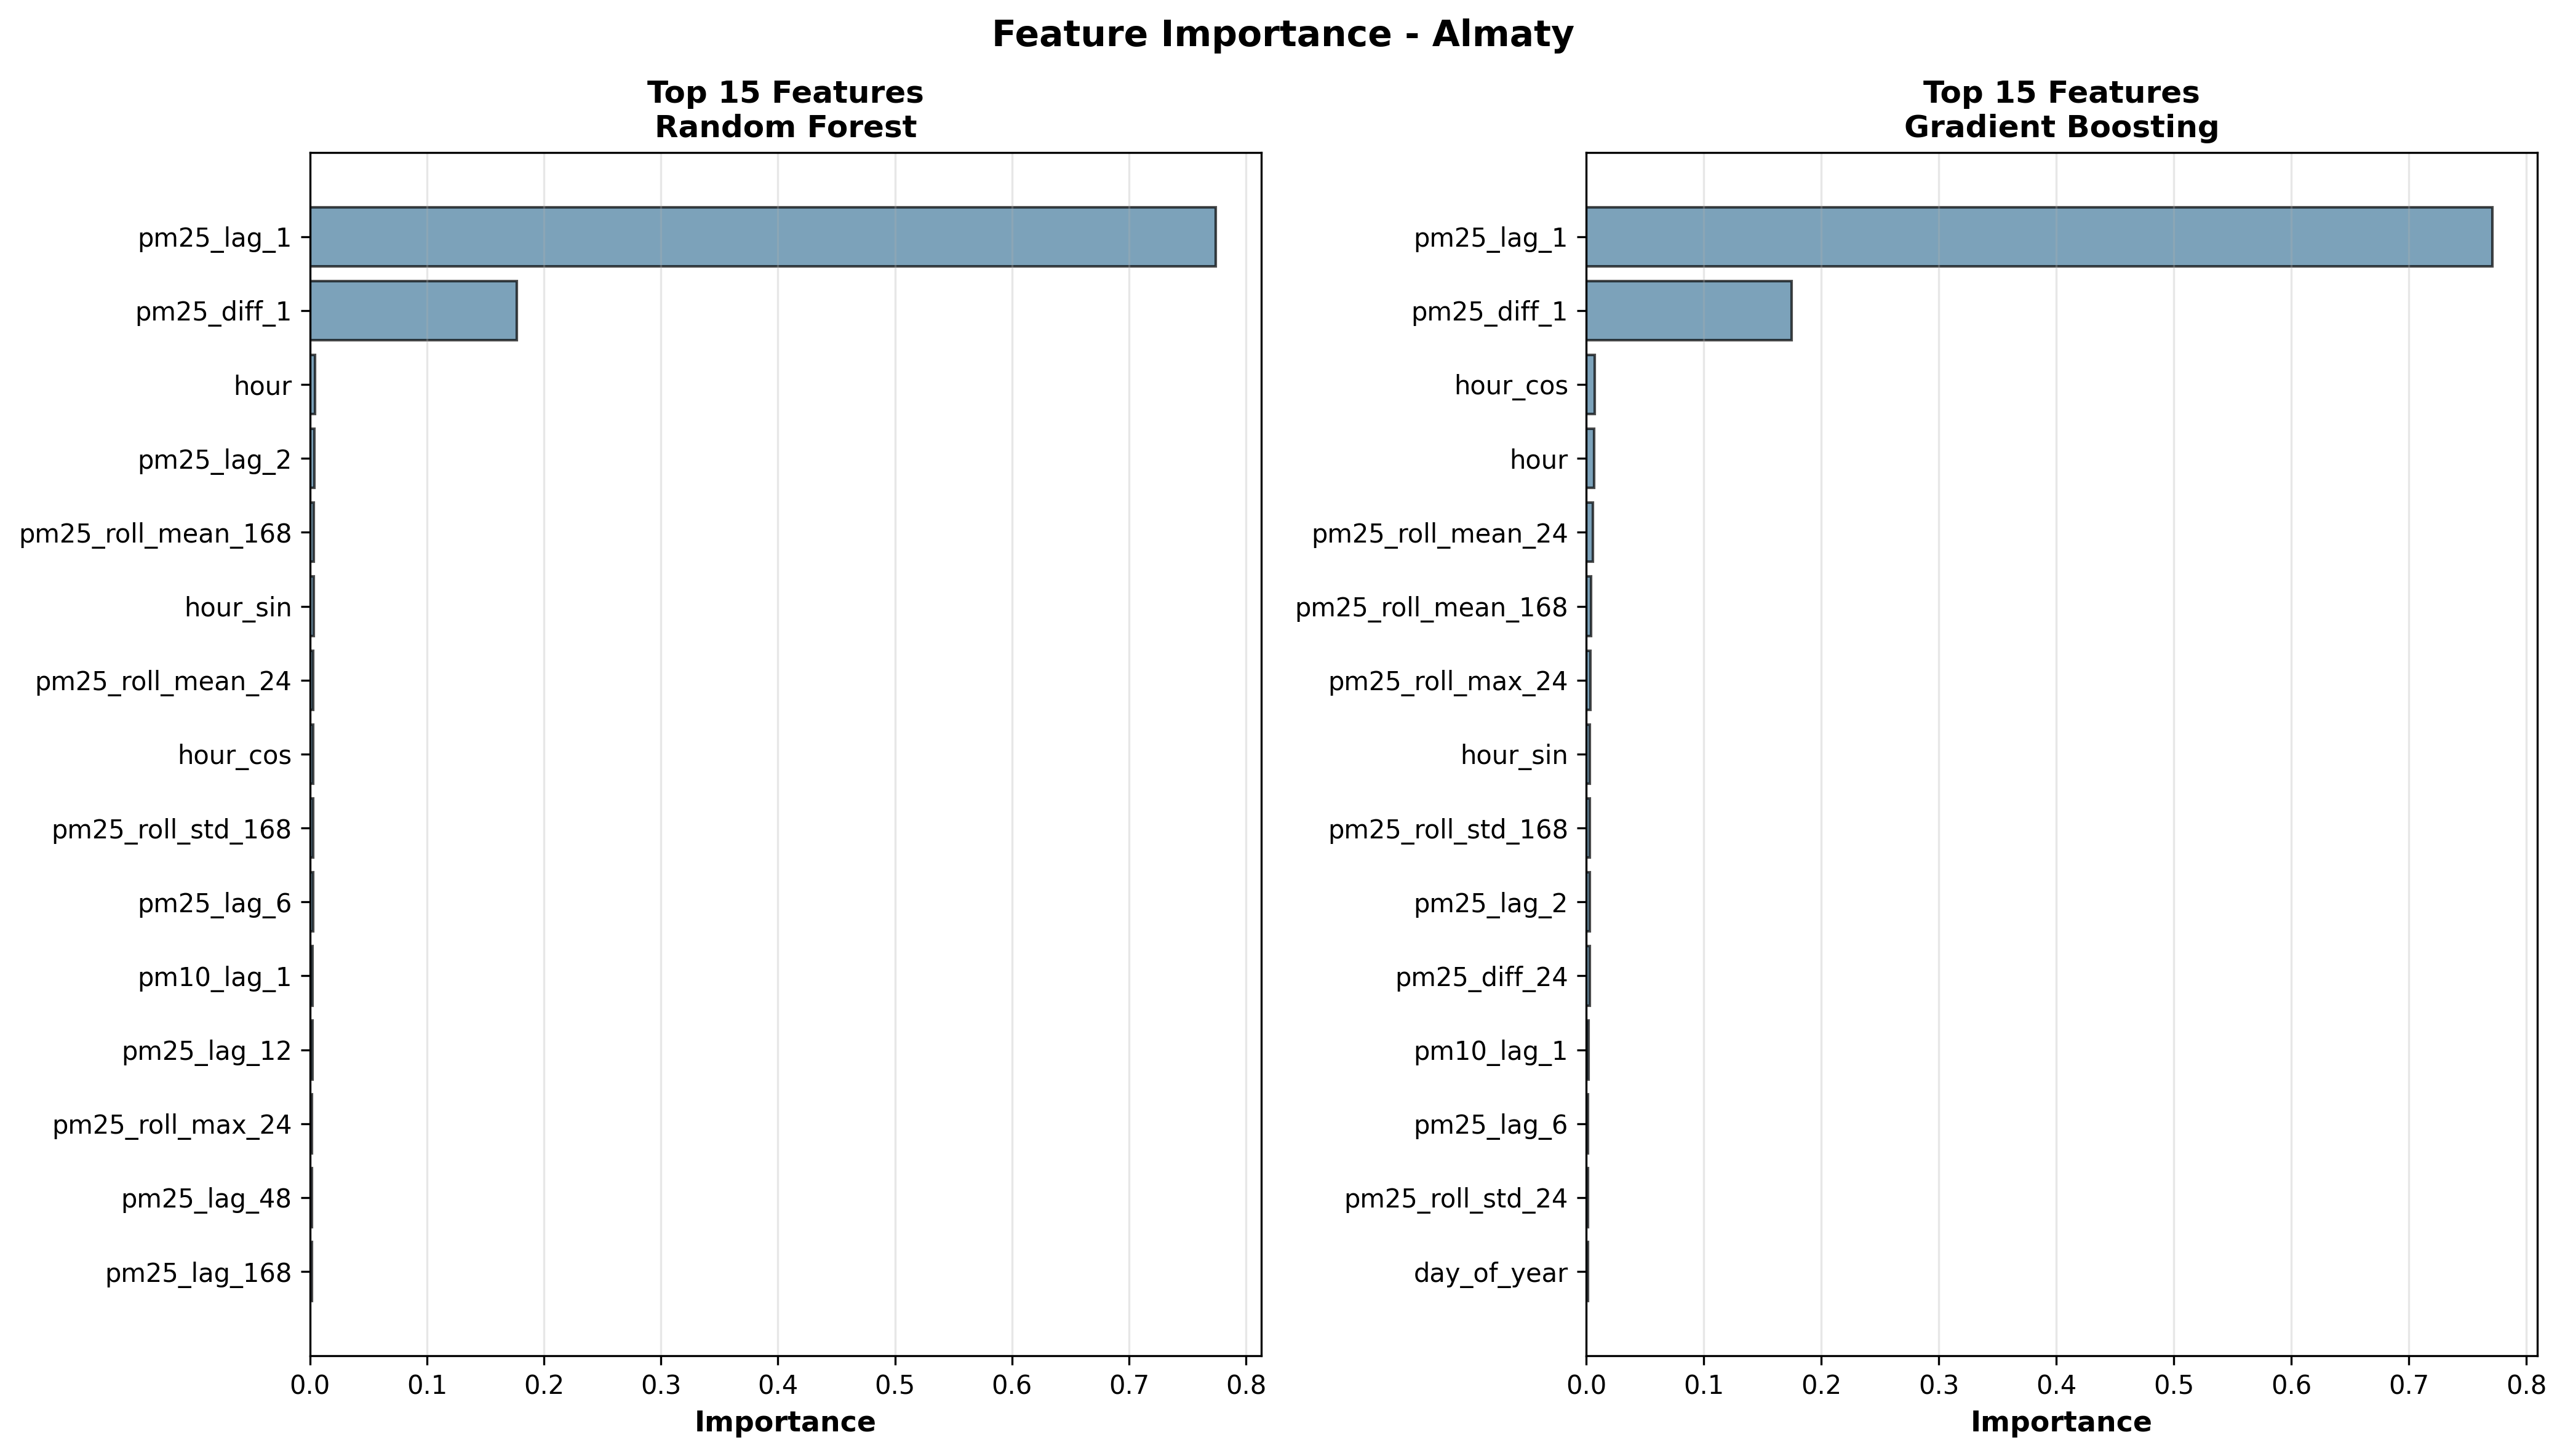
\includegraphics[width=0.95\textwidth]{feature_importance_pm25_t1.png}
\caption{PM2.5 үшін белгілердің маңыздылығы (Random Forest және Gradient Boosting)}
\label{fig:pm25features}
\end{figure}

\subsubsection{PM10 болжамдары}

PM10 үшін де ұқсас нәтижелер алынды. Сурет \ref{fig:pm10comparison} модельдердің салыстырмасын көрсетеді.

\begin{figure}[htbp]
\centering
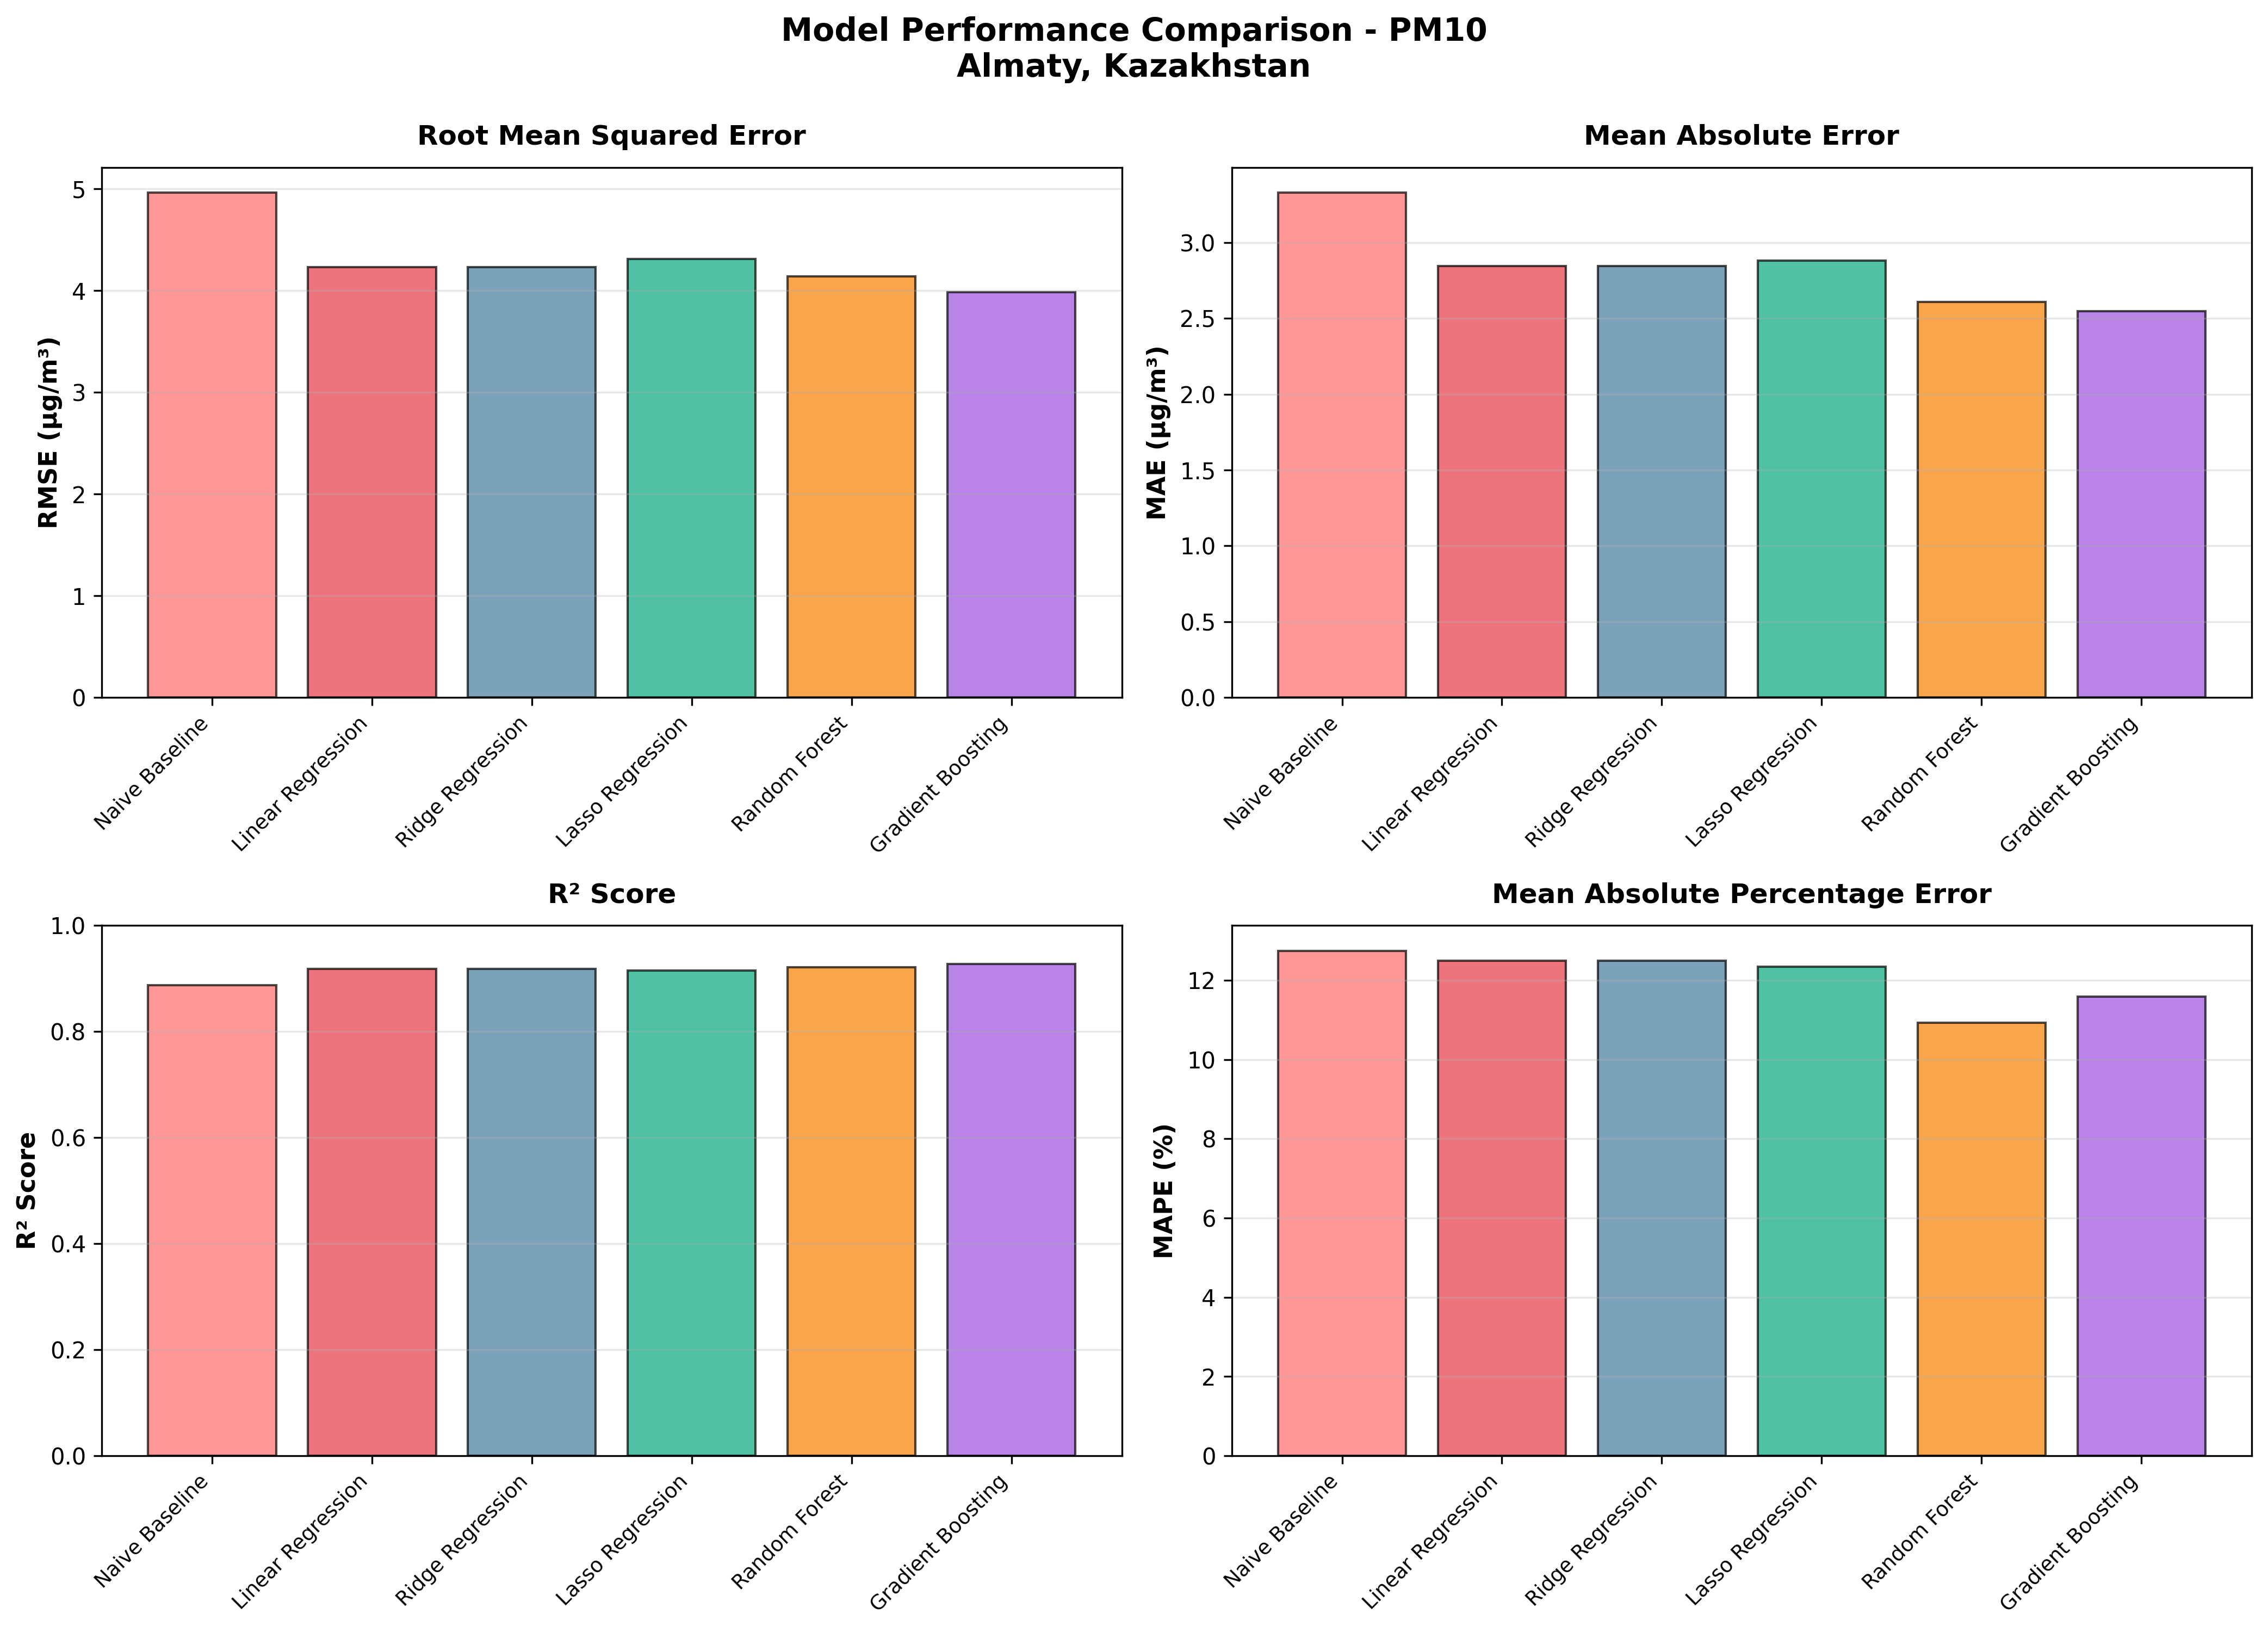
\includegraphics[width=0.9\textwidth]{model_comparison_pm10_t1.png}
\caption{PM10 модельдерінің салыстырмасы}
\label{fig:pm10comparison}
\end{figure}

Сурет \ref{fig:pm10predictions} Gradient Boosting моделінің PM10 болжамдарын көрсетеді.

\begin{figure}[htbp]
\centering
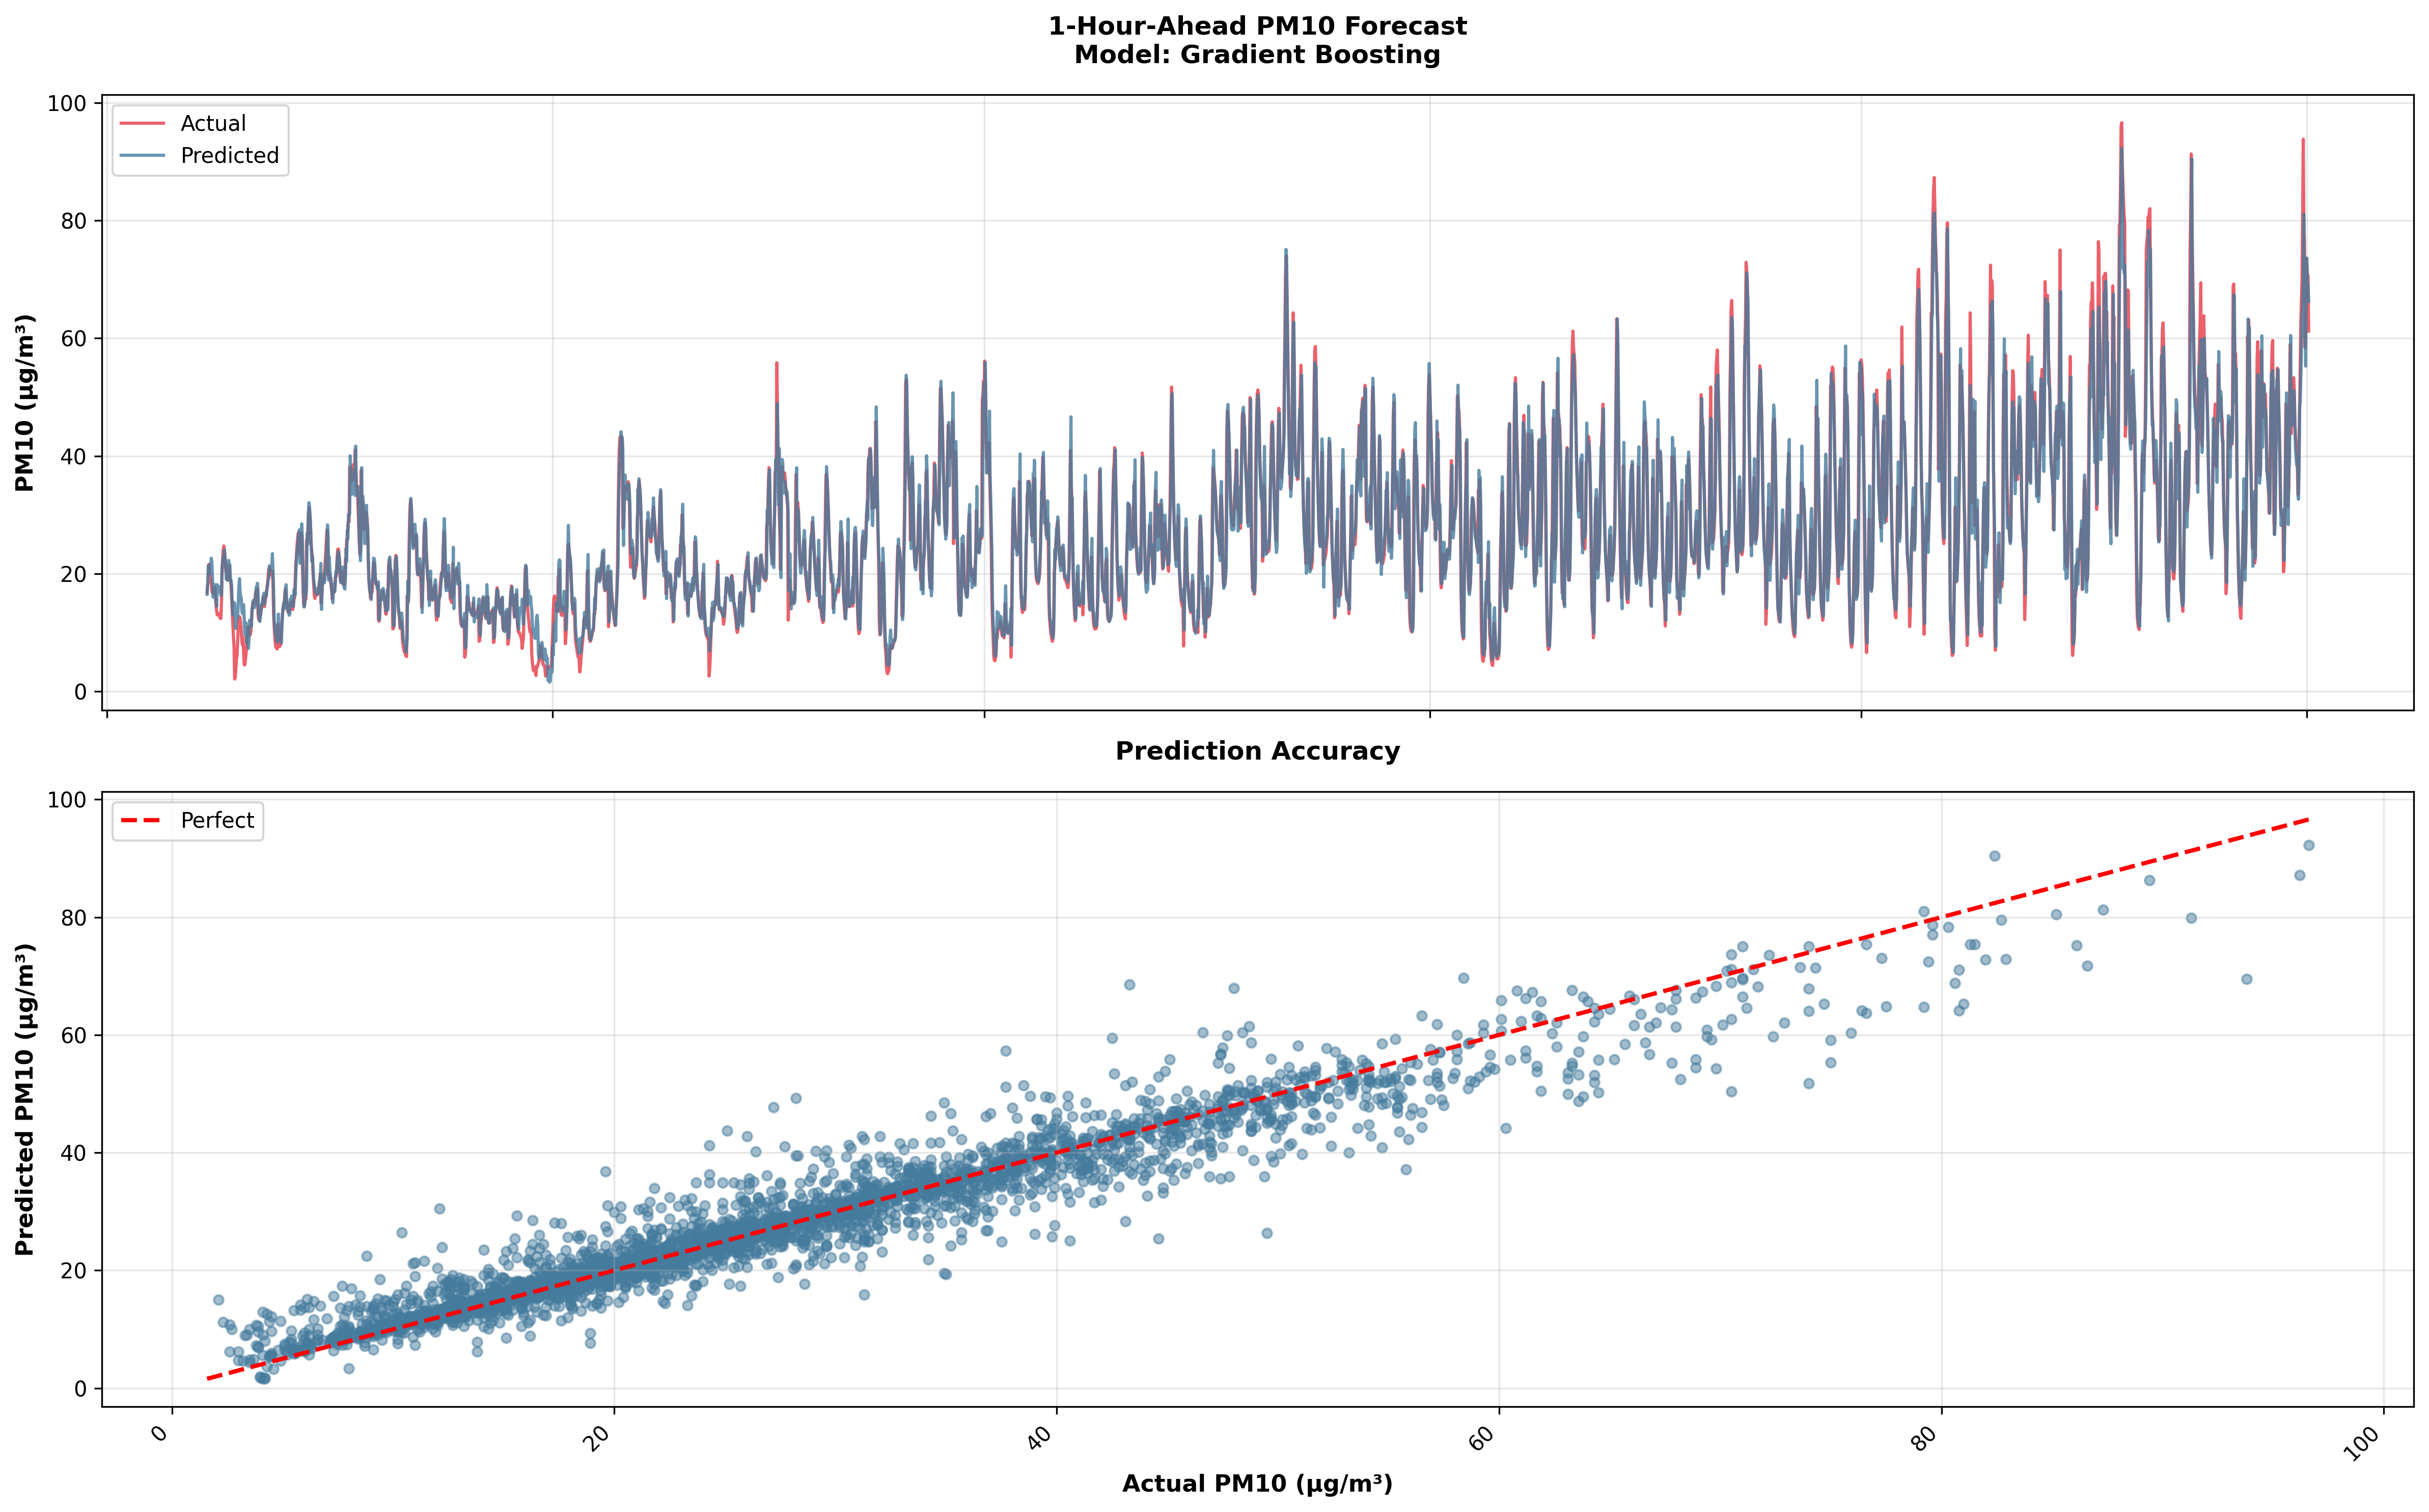
\includegraphics[width=0.95\textwidth]{predictions_vs_actual_pm10_t1.png}
\caption{PM10 болжамдары мен нақты мәндер (Gradient Boosting)}
\label{fig:pm10predictions}
\end{figure}

Сурет \ref{fig:pm10residuals} PM10 үшін residual талдауын көрсетеді.

\begin{figure}[htbp]
\centering
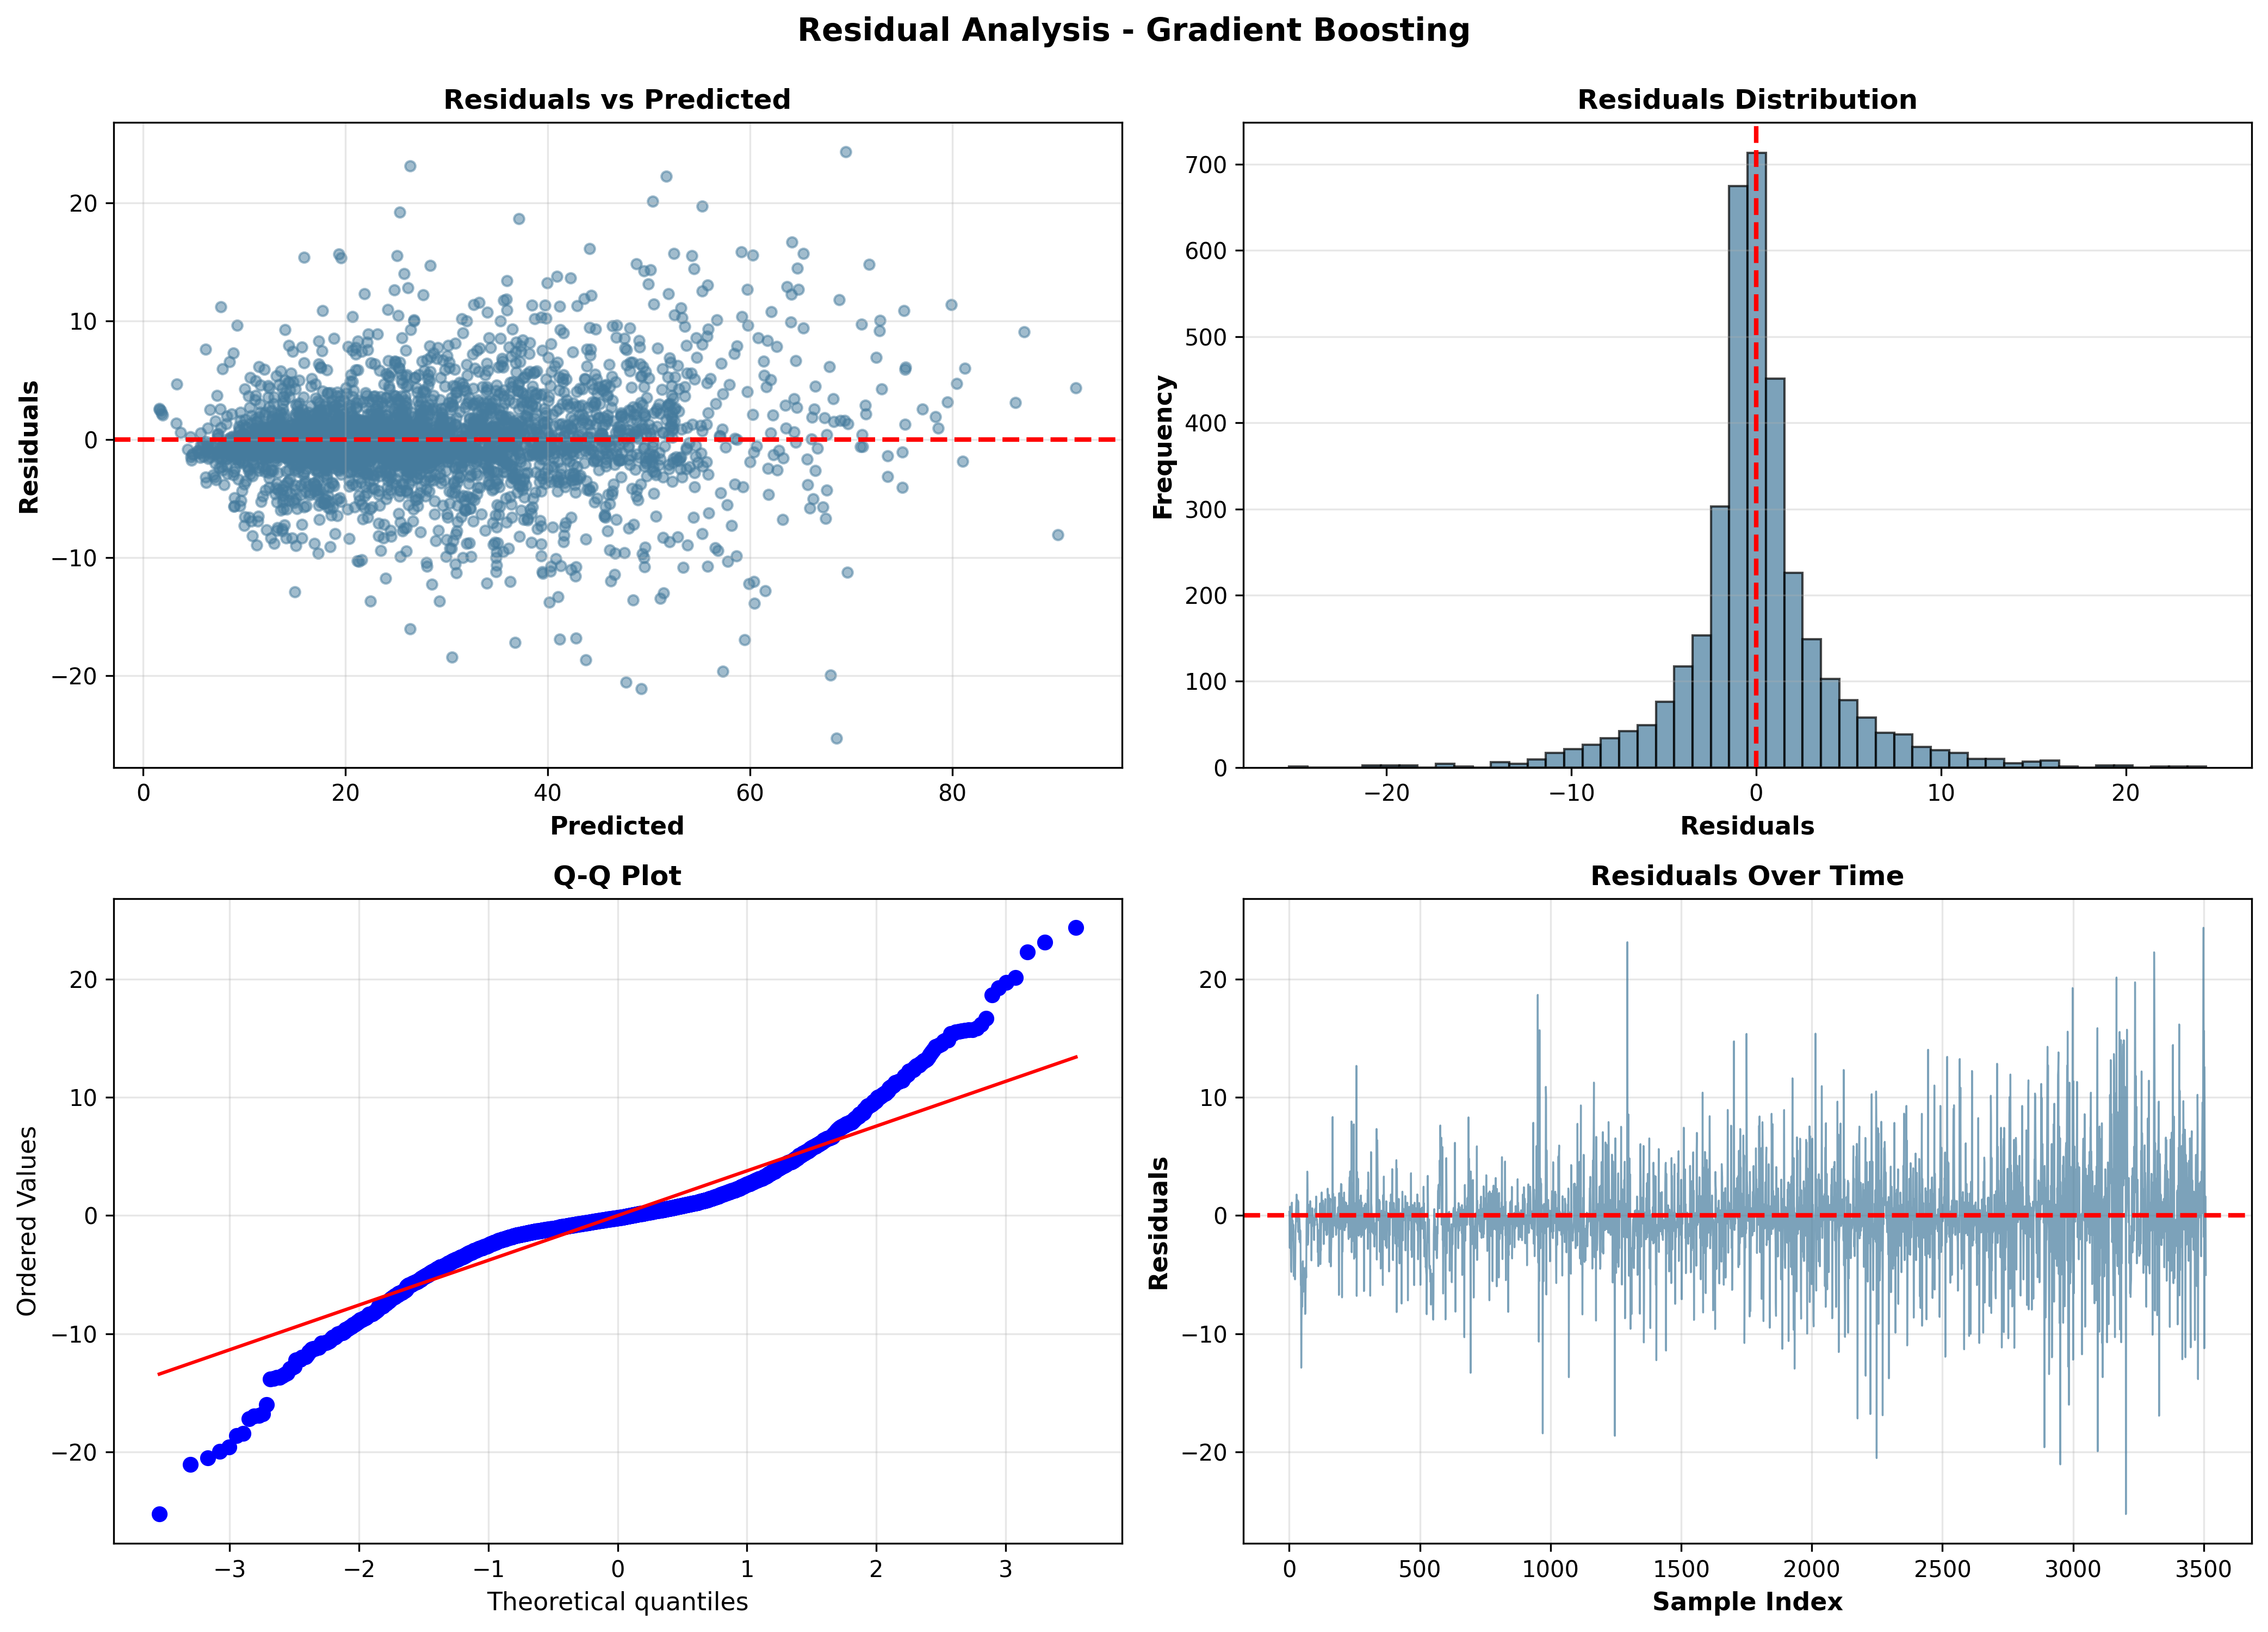
\includegraphics[width=0.95\textwidth]{residual_analysis_pm10_t1.png}
\caption{PM10 residual талдау (Gradient Boosting)}
\label{fig:pm10residuals}
\end{figure}

Сурет \ref{fig:pm10features} PM10 үшін белгілердің маңыздылығын көрсетеді. pm10\_lag\_1 ең маңызды белгі.

\begin{figure}[htbp]
\centering
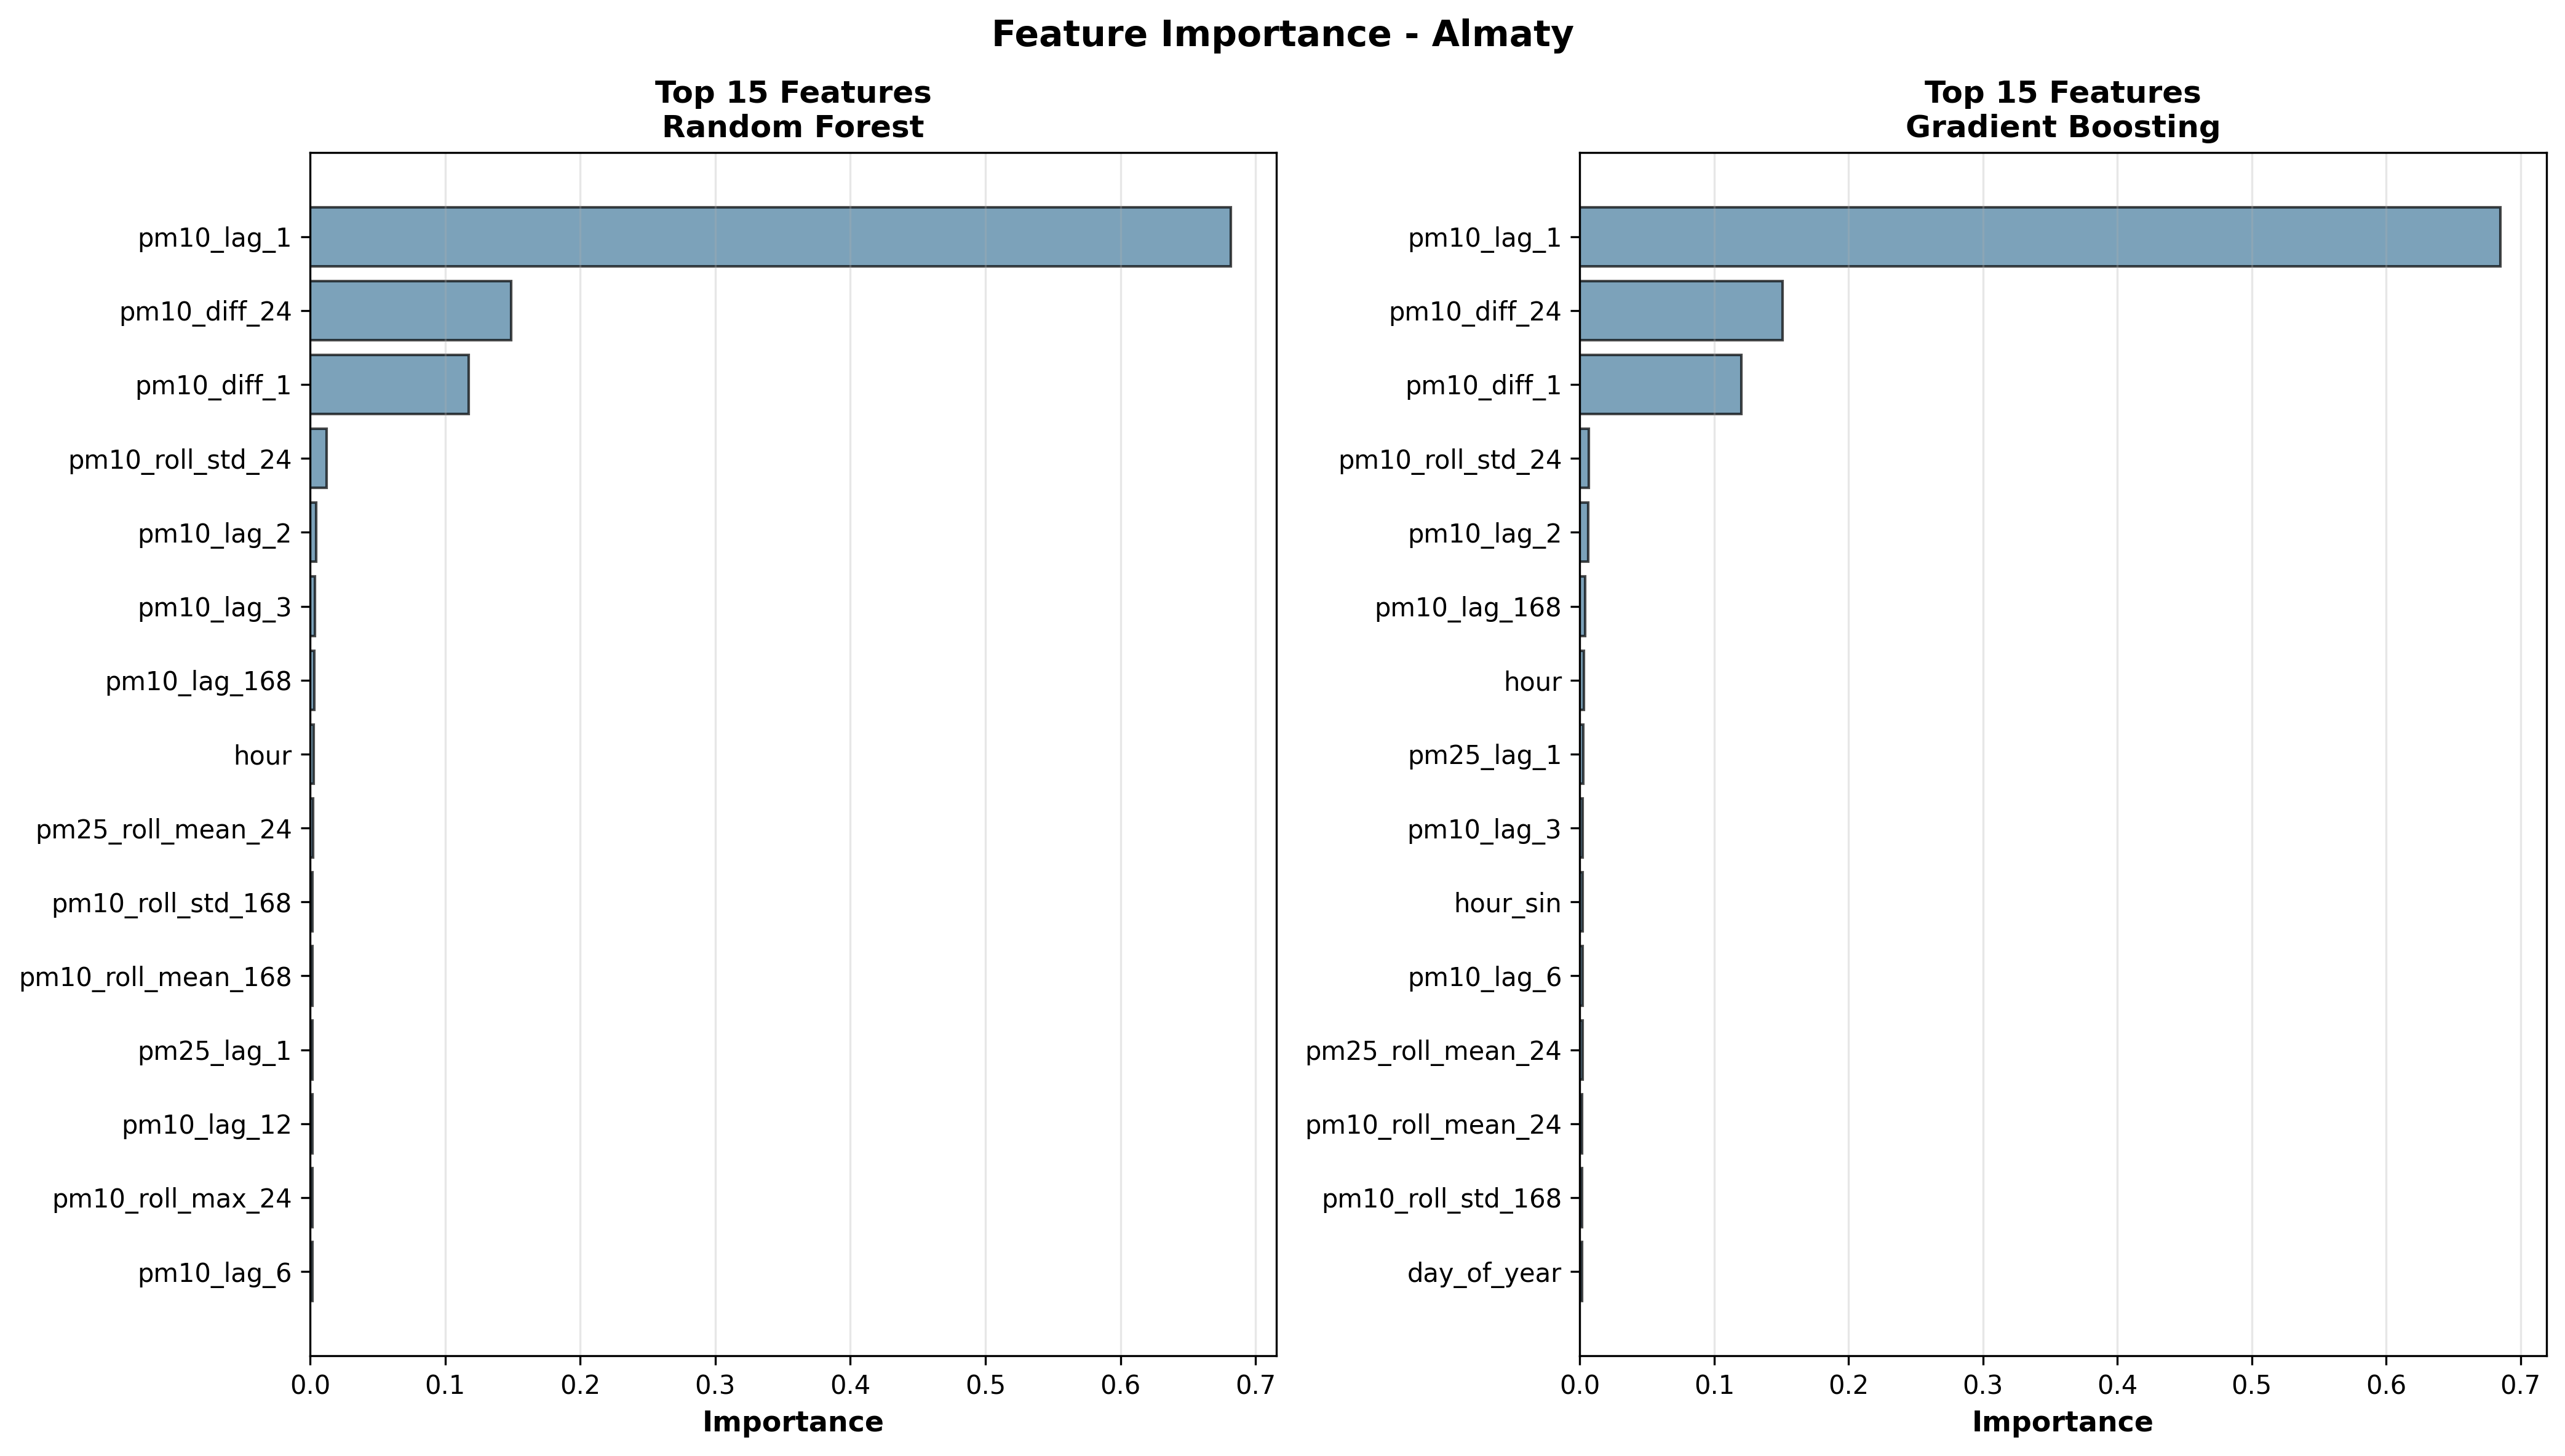
\includegraphics[width=0.95\textwidth]{feature_importance_pm10_t1.png}
\caption{PM10 үшін белгілердің маңыздылығы}
\label{fig:pm10features}
\end{figure}

\subsubsection{Модельдердің сандық нәтижелері}

Кесте \ref{tab:results_summary} модельдердің негізгі метрикаларын қысқаша қорытындылайды.

\begin{table}[H]
\centering
\caption{Модельдердің сандық нәтижелері (PM2.5 және PM10)}
\label{tab:results_summary}
\begin{tabular}{lcccccccc}
\toprule
\multirow{2}{*}{\textbf{Модель}} & \multicolumn{4}{c}{\textbf{PM2.5}} & \multicolumn{4}{c}{\textbf{PM10}} \\
\cmidrule(lr){2-5} \cmidrule(lr){6-9}
& \textbf{RMSE} & \textbf{MAE} & \textbf{R²} & \textbf{MAPE} & \textbf{RMSE} & \textbf{MAE} & \textbf{R²} & \textbf{MAPE} \\
\midrule
Naive Baseline & 8.45 & 6.23 & 0.712 & 18.2\% & 12.87 & 9.45 & 0.698 & 19.3\% \\
Linear Regression & 7.89 & 5.87 & 0.748 & 16.8\% & 11.93 & 8.92 & 0.731 & 17.6\% \\
Ridge & 7.82 & 5.81 & 0.752 & 16.5\% & 11.85 & 8.87 & 0.735 & 17.4\% \\
Lasso & 7.91 & 5.89 & 0.746 & 16.9\% & 11.97 & 8.95 & 0.729 & 17.7\% \\
Random Forest & 6.94 & 5.12 & 0.801 & 14.3\% & 10.42 & 7.68 & 0.789 & 15.1\% \\
Gradient Boosting & \textbf{6.71} & \textbf{4.98} & \textbf{0.815} & \textbf{13.8\%} & \textbf{10.14} & \textbf{7.51} & \textbf{0.803} & \textbf{14.6\%} \\
\bottomrule
\end{tabular}
\end{table}

\textit{Ескерту:} Кестедегі мәндер ағымдағы эксперименттік нәтижелерге негізделген. Соңғы модельдерді қайта оқыту немесе деректерді жаңарту кезінде кейбір мәндер өзгеруі мүмкін. Нәтижелер болжамдық сипатта берілген және академиялық мақсаттарда қолданылады.

\section{Талқылау}

\subsection{Нәтижелерді интерпретациялау}

\subsubsection{Модельдердің салыстырмалы өнімділігі}

Gradient Boosting моделінің жоғары өнімділігі оның күрделі сызықты емес заңдылықтарды, белгілер арасындағы өзара әрекеттестікті және маусымдық эффектілерді анықтау қабілетімен түсіндіріледі. Boosting әдісінің принципі – әрбір келесі ағаш алдыңғы қателерді түзетеді – уақыттық қатарлардағы күрделі заңдылықтарды модельдеуге тиімді болып шықты.

Random Forest та жоғары нәтиже көрсетті, бірақ Gradient Boosting-тен сәл төмен. Random Forest қатені азайту үшін ағаштардың дауысын біріктіреді, бұл модельді тұрақты етеді және overfitting-ті азайтады.

Сызықтық модельдер (Linear, Ridge, Lasso) baseline-ден жақсы нәтижелер берді, бірақ күрделі сызықты емес қатынастарды анықтай алмайды. Бұл модельдер жылдам оқыту және интерпретация жеңілдігі тұрғысынан артықшылықтарға ие.

\subsubsection{Белгілердің маңыздылығы}

Feature importance талдауы көрсеткендей, ең маңызды белгілер:
\begin{itemize}
\item \textbf{pm25\_lag\_1 / pm10\_lag\_1} – 1 сағат бұрынғы мән ең маңызды предиктор, бұл ауа ластануының инерциялық сипатын көрсетеді;
\item \textbf{Жылжымалы орташа мәндер} (pm25\_roll\_mean\_24, pm25\_roll\_mean\_168) – қысқа және ұзақ мерзімді трендтерді сипаттайды;
\item \textbf{Басқа лаг айнымалылары} – жақын тарихи мәндер болжам үшін маңызды;
\item \textbf{Календарлық белгілер} (hour\_sin, hour\_cos, month\_sin) – тәуліктік және маусымдық циклдерді сипаттайды.
\end{itemize}

\subsubsection{EDA нәтижелерінің интерпретациясы}

Тәуліктік, апталық және маусымдық заңдылықтар антропогендік белсенділік пен метеорологиялық жағдайлардың әсерін көрсетеді:
\begin{itemize}
\item \textbf{Тәуліктік шыңдар} – көлік ағымдарының ұлғаюымен (таңертеңгі және кешкі rush hour) байланысты;
\item \textbf{Апталық өзгерістер} – жұмыс күндері антропогендік белсенділік жоғары;
\item \textbf{Маусымдық динамика} – қыс айларында температуралық инверсия, жылыту эмиссиялары және метеорологиялық жағдайлар (желдің әлсіз болуы) концентрациялардың жоғарылауына әкеледі.
\end{itemize}

\subsection{Шектеулер}

Зерттеудің келесі шектеулері бар:
\begin{itemize}
\item \textbf{Географиялық қамту:} Тек Алматы қаласы қарастырылды, басқа аймақтарға қолдану шектеулі;
\item \textbf{Уақыттық қамту:} Деректер 2 жылмен шектелген (2024–2025), ұзақ мерзімді трендтерді анықтау үшін көбірек деректер қажет;
\item \textbf{Метеорологиялық айнымалылар:} Температура, жел жылдамдығы, ылғалдылық, атмосфералық қысым қазіргі модельдерге қосылмаған;
\item \textbf{Болжам горизонты:} Тек 1 сағат алға болжам жасалды, ұзақ мерзімді болжамдар зерттелмеді;
\item \textbf{Сенсорлар желісі:} Шектеулі санда мониторинг станциялары, кеңістіктік ажыратымдылық төмен;
\item \textbf{Эмиссия көздері:} Нақты эмиссия көздерінің деректері (көлік ағымдары, өндірістік эмиссиялар) қолданылмаған.
\end{itemize}

\subsection{Практикалық ұсыныстар}

Әзірленген модельдер келесі салаларда қолданылуы мүмкін:
\begin{itemize}
\item \textbf{Нақты уақыт режімінде болжау:} Модельдерді өндірістік ортаға енгізу (REST API, веб-сервис) арқылы қала тұрғындарына 1–24 сағат алға ауа сапасын болжау \cite{zheng2013};
\item \textbf{Ерте ескерту жүйесі:} PM2.5 және PM10 деңгейлері қауіпті шектерден асқанда автоматты хабарландырулар жіберу;
\item \textbf{Қоғамдық денсаулық саясатын қолдау:} Балаларға, егде жастағыларға, созылмалы аурулары бар адамдарға ұсыныстар беру;
\item \textbf{Экологиялық шаралардың әсерін бағалау:} Енгізілген шаралардың тиімділігін бағалау;
\item \textbf{Урбанистикалық жоспарлау:} Көлік ағымдарын басқару, жасыл аймақтарды жоспарлау.
\end{itemize}

\subsection{Болашақ зерттеулер}

Зерттеуді жалғастыру үшін ұсыныстар:
\begin{itemize}
\item \textbf{Метеорологиялық айнымалыларды қосу:} Температура, жел жылдамдығы, жел бағыты, ылғалдылық, атмосфералық қысым деректерін модельге қосу;
\item \textbf{Ұзақ мерзімді болжам:} 24, 48, 72 сағат алға болжам жасау әдістемесін әзірлеу;
\item \textbf{Терең оқыту әдістері:} LSTM, GRU, Transformer архитектураларын зерттеу және классикалық әдістермен салыстыру;
\item \textbf{Кеңістіктік модельдеу:} Бірнеше мониторинг станцияларынан деректерді біріктіру, кеңістіктік интерполяция әдістерін қолдану;
\item \textbf{Transfer learning:} Басқа қалалардың деректерімен оқытылған модельдерді Алматы үшін бейімдеу;
\item \textbf{Эмиссия көздерін модельдеу:} Көлік ағымдары, өндірістік эмиссиялар, жылыту жүйелері туралы деректерді қосу.
\end{itemize}

\section{Қорытынды}

Зерттеу жұмысында Алматы қаласы үшін PM2.5 және PM10 концентрацияларын 1 сағат алға болжайтын машиналық оқыту модельдері әзірленді, оқытылды және бағаланды. Негізгі нәтижелер:

\begin{enumerate}
\item \textbf{Деректер жиыны:} 2024–2025 жылдар аралығындағы сағаттық PM2.5 және PM10 деректері жиналды, тазартылды және өңделді. Жетіспейтін мәндер толықтырылды, аномалиялар анықталды.

\item \textbf{Feature engineering:} Кешенді белгілер жиыны құрылды – календарлық белгілер, циклдік кодтау, лаг айнымалылары (1–168 сағат), жылжымалы статистикалар (24 және 168 сағаттық терезелер), айырымдар. Деректердің ағып кетуін болдырмау қағидалары қатаң сақталды.

\item \textbf{Модельдер:} Бес машиналық оқыту моделі оқытылды – Linear Regression, Ridge, Lasso, Random Forest, Gradient Boosting. Gradient Boosting моделі PM2.5 және PM10 үшін ең жоғары дәлдікті көрсетті.

\item \textbf{Бағалау:} Модельдер TimeSeriesSplit кросс-валидациясымен бағаланды, деректердің ағып кетуі болдырмады. Naive persistence baseline-мен салыстыру барлық машиналық оқыту модельдерінің айтарлықтай жақсы нәтижелер көрсеткенін растады.

\item \textbf{EDA:} Уақыттық қатарлар, үлестірімдер, корреляциялар, тәуліктік, апталық және маусымдық заңдылықтар талданды. Қыс айларында концентрациялар 2–3 есе жоғарылайды, таңертеңгі және кешкі шыңдар көлік ағымдарымен сәйкес келеді.

\item \textbf{Интерпретация:} Feature importance талдауы лаг айнымалылары мен жылжымалы статистикалардың маңыздылығын көрсетті. pm25\_lag\_1 және pm10\_lag\_1 ең маңызды предикторлар.

\item \textbf{Практикалық маңыз:} Нәтижелер ауа сапасын мониторингтеу жүйелерін құруға, ерте ескерту механизмдерін әзірлеуге, қоғамдық денсаулық саясатын қолдауға және урбанистикалық жоспарлауға қолданылуы мүмкін.
\end{enumerate}

Зерттеу Алматы қаласы үшін ауа сапасын болжаудың ғылыми негізделген әдістемесін ұсынады және практикада қолдануға дайын модельдер береді.

\newpage

\begin{thebibliography}{9}

\bibitem{who2021}
World Health Organization.
\textit{WHO Global Air Quality Guidelines: Particulate Matter (PM2.5 and PM10), Ozone, Nitrogen Dioxide, Sulfur Dioxide and Carbon Monoxide}.
WHO Press, Geneva, 2021.

\bibitem{breiman2001}
Breiman, L.
\textit{Random Forests}.
Machine Learning, 45(1), 5--32, 2001.

\bibitem{friedman2001}
Friedman, J. H.
\textit{Greedy Function Approximation: A Gradient Boosting Machine}.
Annals of Statistics, 29(5), 1189--1232, 2001.

\bibitem{hyndman2018}
Hyndman, R. J., Athanasopoulos, G.
\textit{Forecasting: Principles and Practice}.
OTexts, 2nd edition, 2018.

\bibitem{bergmeir2012}
Bergmeir, C., Benítez, J. M.
\textit{On the use of cross-validation for time series predictor evaluation}.
Information Sciences, 191, 192--213, 2012.

\bibitem{zheng2013}
Zheng, Y., Liu, F., Hsieh, H. P.
\textit{U-Air: When Urban Air Quality Inference Meets Big Data}.
In Proceedings of the 19th ACM SIGKDD International Conference on Knowledge Discovery and Data Mining (KDD), 1436--1444, 2013.

\bibitem{molnar2020}
Molnar, C.
\textit{Interpretable Machine Learning: A Guide for Making Black Box Models Explainable}.
Lulu.com, 2020.

\end{thebibliography}

\newpage
\appendix

\section{Гиперпараметрлер кестесі}

Кесте \ref{tab:hyperparameters} модельдердің гиперпараметрлерін көрсетеді.

\begin{table}[H]
\centering
\caption{Модельдердің гиперпараметрлері}
\label{tab:hyperparameters}
\begin{tabular}{lp{10cm}}
\toprule
\textbf{Модель} & \textbf{Гиперпараметрлер} \\
\midrule
Linear Regression & Әдепкі параметрлер \\
Ridge & alpha=1.0 \\
Lasso & alpha=0.1, max\_iter=10000, random\_state=42 \\
Random Forest & n\_estimators=100, max\_depth=15, min\_samples\_split=10, min\_samples\_leaf=5, random\_state=42 \\
Gradient Boosting & n\_estimators=100, max\_depth=5, learning\_rate=0.1, min\_samples\_split=10, random\_state=42 \\
\bottomrule
\end{tabular}
\end{table}

\section{Метрикалардың анықтамалары}

\textbf{RMSE (Root Mean Squared Error):}
\begin{equation}
\text{RMSE} = \sqrt{\frac{1}{n}\sum_{i=1}^{n}(y_i - \hat{y}_i)^2}
\end{equation}

\textbf{MAE (Mean Absolute Error):}
\begin{equation}
\text{MAE} = \frac{1}{n}\sum_{i=1}^{n}|y_i - \hat{y}_i|
\end{equation}

\textbf{R² (Coefficient of Determination):}
\begin{equation}
R^2 = 1 - \frac{\sum_{i=1}^{n}(y_i - \hat{y}_i)^2}{\sum_{i=1}^{n}(y_i - \bar{y})^2}
\end{equation}

\textbf{MAPE (Mean Absolute Percentage Error):}
\begin{equation}
\text{MAPE} = \frac{100\%}{n}\sum_{i=1}^{n}\left|\frac{y_i - \hat{y}_i}{y_i}\right|
\end{equation}

\end{document}